%Este trabalho está licenciado sob a Licença Atribuição-CompartilhaIgual 4.0 Internacional Creative Commons. Para visualizar uma cópia desta licença, visite http://creativecommons.org/licenses/by-sa/4.0/deed.pt_BR ou mande uma carta para Creative Commons, PO Box 1866, Mountain View, CA 94042, USA.

\documentclass[12pt]{book}

\input ../preambulo.tex

\makeindex

\begin{document}

\frontmatter

\title{Matemática numérica}
\author{Pedro H A Konzen}
\date{\today}
\ifishtml
\else
\addcontentsline{toc}{chapter}{Capa}
\fi

\maketitle

%Este trabalho está licenciado sob a Licença Atribuição-CompartilhaIgual 4.0 Internacional Creative Commons. Para visualizar uma cópia desta licença, visite http://creativecommons.org/licenses/by-sa/4.0/ ou mande uma carta para Creative Commons, PO Box 1866, Mountain View, CA 94042, USA.

\chapter*{Licença}\label{licenca}
\addcontentsline{toc}{chapter}{Licença}

Este trabalho está licenciado sob a Licença Atribuição-CompartilhaIgual 4.0 Internacional Creative Commons. Para visualizar uma cópia desta licença, visite http://creativecommons.org/licenses/by-sa/4.0/deed.pt\_BR ou mande uma carta para Creative Commons, PO Box 1866, Mountain View, CA 94042, USA.

%Este trabalho está licenciado sob a Licença Atribuição-CompartilhaIgual 4.0 Internacional Creative Commons. Para visualizar uma cópia desta licença, visite http://creativecommons.org/licenses/by-sa/4.0/deed.pt_BR ou mande uma carta para Creative Commons, PO Box 1866, Mountain View, CA 94042, USA.

\chapter*{Prefácio}\label{prefacio}
\addcontentsline{toc}{chapter}{Prefácio}

Nestas notas de aula são abordados temas introdutórios de análise matemática na reta. No primeiro capítulo, são discutidos alguns tópicos sobre funções e topologia, os quais são fundamentais nos desenvolvimentos demais capítulos. Na sequência são discutidos os conceitos e aplicações sobre limites e continuidade de funções, derivação e integração de funções, bem como sequências e séries de funções.

Agradeço aos(às) estudantes que assiduamente contribuem com correções, sugestões e críticas em prol do desenvolvimento deste material didático.

\begin{flushright}
  Pedro H A Konzen
\end{flushright}

\tableofcontents
\addcontentsline{toc}{chapter}{Sumário}

\mainmatter

%Este trabalho está licenciado sob a Licença Atribuição-CompartilhaIgual 4.0 Internacional Creative Commons. Para visualizar uma cópia desta licença, visite http://creativecommons.org/licenses/by-sa/4.0/deed.pt_BR ou mande uma carta para Creative Commons, PO Box 1866, Mountain View, CA 94042, USA.

\chapter{Introdução}\label{cap:introducao}
\thispagestyle{fancy}

\emconstrucao
%Este trabalho está licenciado sob a Licença Atribuição-CompartilhaIgual 4.0 Internacional Creative Commons. Para visualizar uma cópia desta licença, visite http://creativecommons.org/licenses/by-sa/4.0/ ou mande uma carta para Creative Commons, PO Box 1866, Mountain View, CA 94042, USA.

\chapter{Aproximação por mínimos quadrados}\label{cap_ajuste}
\thispagestyle{fancy}

\section{Problemas lineares}\label{cap_ajuste_sec_prob_lin}

Dado um conjunto de $n$ pontos $\{(x_i,y_i)\}_{i=1}^n$, $x_i\neq x_j$ para $i\neq j$, e uma família de $m \leq n$ funções $\{f_i(x)\}_{i=1}^m$, o problema linear de aproximação por mínimos quadrados consiste em determinar os $m$ coeficientes $\{c_i\}_{i=1}^m$ tal que a função
\begin{align}    
  f(x;c) &= \sum_{j=1}^m c_jf_j(x) \\
         &= c_1f_1(x) + c_2f_2(x) + c_3f_3(x) + \cdots + c_mf_m(x)
\end{align}
aproxime o conjunto de pontos dados no sentido de mínimos quadrados, i.e. o vetor dos coeficientes $c = (c_1, c_2, \dotsc, c_m)$ é solução do seguinte problema linear de minimização
\begin{equation}
  \min_{c} \left\{E:= \sum_{i=1}^n (y_i - f(x_i;c))^2\right\}.
\end{equation}

A fim de trabalharmos com uma notação mais compacta, definimos o resíduo $r(c) = (r_1(c), r_2(c), \dotsc, r_n(c))$, onde $r_i(c) := y_i - f(x_i)$ e $c = (c_1, c_2, \dotsc, c_m)$. Com esta notação, o problema de mínimos quadrados se resume a resolver
\begin{equation}\label{eq:pmq}
  \min_{c} \{E := \|r(c)\|_2^2\}.
\end{equation}

\subsection{Método das equações normais}

A fim de resolver o problema de mínimos quadrados~\eqref{eq:pmq}, observamos que o erro quadrático
\begin{align}
  E &= \|r(c)\|_2^2 \\
    &= \sum_{i=1}^n r_i(c)^2 \\
    &= \sum_{i=1}^n \left(y_i - f(x_i;c)\right)^2 \\
    &= \sum_{i=1}^n \left(y_i - \sum_{j=1}^m c_jf_j(x_i)\right)^2 \\
    &= \|y - Ac\|_2^2,
\end{align}
onde $y = (y_1, y_2, \dotsc, y_n)$ e
\begin{equation}
  A :=
  \begin{bmatrix}
    f_1(x_1) & f_2(x_1) & \cdots & f_m(x_1) \\
    f_1(x_2) & f_2(x_2) & \cdots & f_m(x_2) \\
    \vdots & \vdots & \vdots & \vdots \\
    f_1(x_n) & f_2(x_n) & \cdots & f_m(x_n)
  \end{bmatrix}.
\end{equation}

Os parâmetros $c_j$ que minimizam o erro $E$ são solução do seguinte sistema de equações
\begin{equation}
  \frac{\p E}{\p c_j} = 2\sum_{i=0}^n r_i(c)\frac{\p}{\p c_j}r_i(c) = 0,
\end{equation}
onde $j=1, 2, \dotsc, m$. Ou, em uma notação mais apropriada,
\begin{align}
  \nabla_c E = 0 &\Leftrightarrow A^Tr(c) = 0\\
  &\Leftrightarrow A^T(y - Ac) = 0\\
  &\Leftrightarrow A^TAc = A^Ty.
\end{align}

Portanto, o problema linear de mínimos quadrados se resume em resolver as chamadas \emph{equações normais}\index{equações normais}
\begin{equation}\label{eq:equacoes_normais}
  A^TAc= A^Ty.
\end{equation}

Logo, o problema linear de mínimos quadrados~\eqref{eq:pmq} reduz-se a resolver o sistema linear \eqref{eq:equacoes_normais} para $c$. Isto nos leva a questão de verificar se $A^TA$ é invertível. De sorte, da disciplina de álgebra linear temos o seguinte teorema.

\begin{teo}
  A matriz $A^TA$ é positiva definida se, e somente se, as colunas de $A$ são linearmente independentes (i.e. $\text{posto}(A)=n$).
\end{teo}
\begin{dem}
  Se as colunas de $A$ são linearmente independentes, então $x\neq 0$ implica $Ax\neq 0$ e, equivalentemente, $x^TA^T\neq 0$. Portanto, $x\neq 0$ implica $x^TA^TAx = \|Ax\|_2^2 > 0$, o que mostra que $A^TA$ é positiva definida.

  Suponhamos, agora, que as colunas de $A$ não são linearmente independentes. Então, existe $x_0\neq 0$ tal que $Ax_0 = 0$. Mas, então, $x_0^TA^TAx_0=0$, o que mostra que $A^TA$ não é positiva definida. 
\end{dem}

Este teorema nos fornece uma condição suficiente para a existência (e unicidade) de solução do problema linear de mínimos quadrados. Mais especificamente, se as colunas da matriz $A$ são linearmente independentes, então os coeficientes da função $f(x)$ que melhor ajustam os pontos dados são
\begin{equation}
  c = (A^TA)^{-1}A^Ty.
\end{equation}

\begin{ex}\normalfont{(Ajuste de polinômios)}\label{ex:ajuste_de_polinomios}
  Considere o problema de ajustar o conjunto de pontos
  \begin{center}
    \begin{tabular}{l|rrrr}
      $i$ & $1$ & $2$ & $3$ & $4$ \\\hline
      $x_i$ & $-1$ & $0$ & $1$ & $1,5$\\
      $y_i$ & $1,2$ & $-0,1$ & $0,7$ & $2,4$\\\hline
    \end{tabular}
  \end{center}
  por um polinômio quadrático da forma
  \begin{equation}
    p(x) = p_1x^2 + p_2x + p_n
  \end{equation}
  no sentido de mínimos quadrados.  

  \begin{figure}[h]
    \centering
    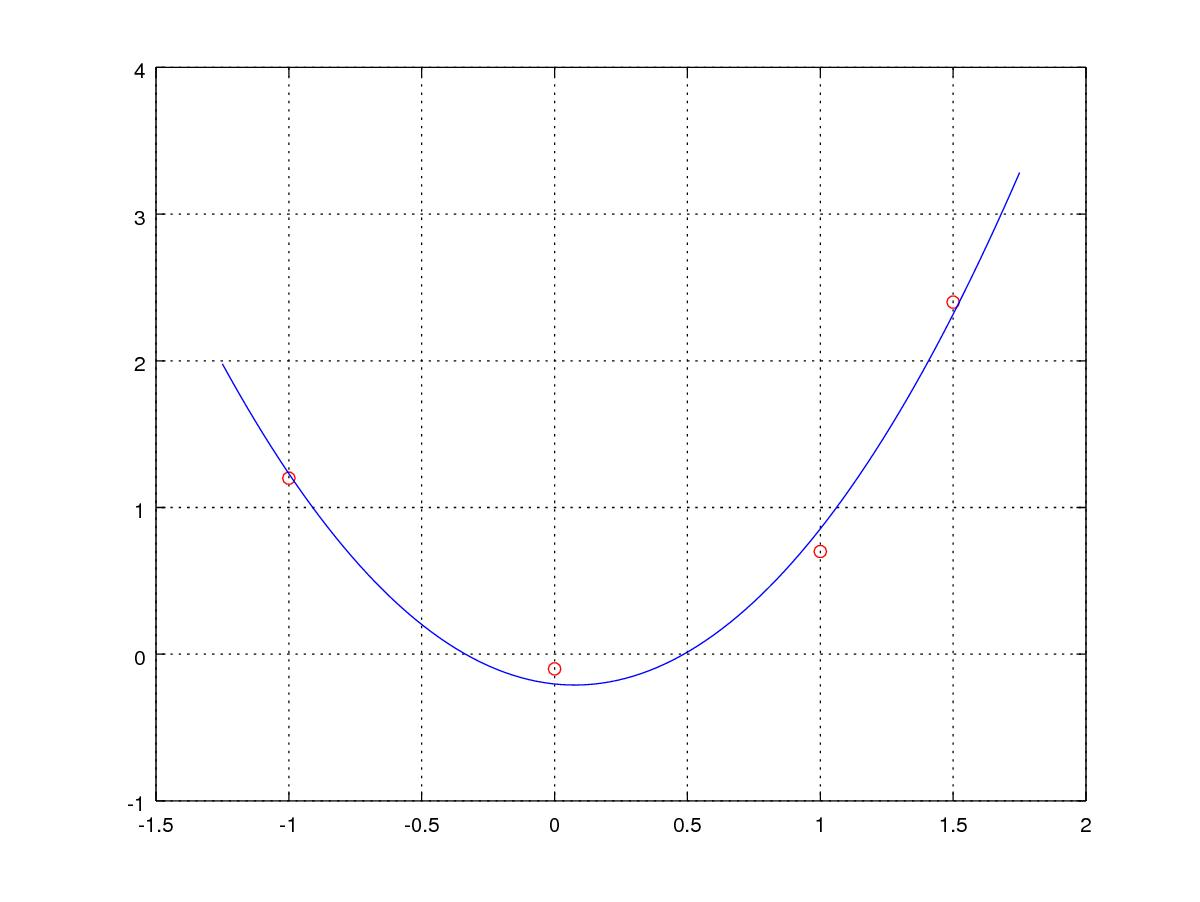
\includegraphics[width=\textwidth]{cap_ajuste/dados/ex_mq_poli/ex_mq_poli}
    \caption{Esboço do polinômio ajustado no Exemplo~\ref{ex:ajuste_de_polinomios}.}
    \label{fig:ex_mq_poli}
  \end{figure}
  
  
  Neste caso, a família de funções do problema de mínimos quadrados é $f_1(x) = x^2$, $f_2(x) = x$ e $f_3(x) = 1$. Assim sendo, os coeficientes $p = (p_1, p_2, p_3)$ são solução do seguinte sistema linear
  \begin{equation}\label{eq:aux3_md}
    A^TAp = A^Ty,
  \end{equation}
  onde $y = (y_1, y_2, y_3)$ e
  \begin{equation}
    A :=
    \begin{bmatrix}
      x_1^2 & x_1 & 1 \\
      x_2^2 & x_2 & 1 \\
      x_3^2 & x_3 & 1 \\
      x_4^2 & x_4 & 1
    \end{bmatrix}.
  \end{equation}
  Emfim, resolvendo as equações normais~\eqref{eq:aux3_md}, obtemos
  \begin{equation}
    p(x) = 1,25x^2 -0,188x - 0,203.
  \end{equation}
  A Figura~\ref{fig:ex_mq_poli} mostra um esboço dos pontos (em vermelho) e do polinômio ajustado (em azul).
  
  \ifisoctave
  Os coeficientes e um esboço do polinômio ajustado podem ser obtidos no \verb+GNU Octave+ com o seguinte código:
\begin{verbatim}
#pontos
x = [-1 0 1 1.5]';
y = [1.2, -0.1, 0.7, 2.4]';

#resol. as eqs. normais
A = [x.^2 x.^1 x.^0];
p = inv(A'*A)*A'*y

#esboco do pol. ajustado
xx = linspace(-1.25,1.75);
plot(x,y,'ro',...
     xx,polyval(p,xx));grid
\end{verbatim}
  \fi
  
\end{ex}


\begin{ex}\normalfont{(Ajuste de curvas)}\label{ex:ajuste_de_curvas}
  Consideremos o mesmo conjunto de pontos do exemplo anterior (Exemplo~\ref{ex:ajuste_de_polinomios}). Aqui, vamos ajustar uma curva da forma
  \begin{equation}
    f(x) = c_1\sen(x) + c_2\cos(x) + c_3
  \end{equation}
no sentido de mínimos quadrados. Para tanto, formamos a matriz
\begin{equation}
  A :=
  \begin{bmatrix}
    \sen(x_1) & \cos(x_1) & 1 \\
    \sen(x_2) & \cos(x_2) & 1 \\
    \sen(x_3) & \cos(x_3) & 1 \\
    \sen(x_4) & \cos(x_4) & 1
  \end{bmatrix}
\end{equation}
  e, então, resolvemos as equações normais $A^TAc = A^Ty$ para o vetor de coeficientes $c=(c_1, c_2)$. Fazendo isso, obtemos $c_1=-0,198$, $c_2=-2,906$ e $c_3=2,662$. A Figura~\ref{fig:ex_mq_curvas} mostra um esboço da curva ajustada (linha azul) aos pontos dados (círculos vermelhos).

  \begin{figure}[h]
    \centering
    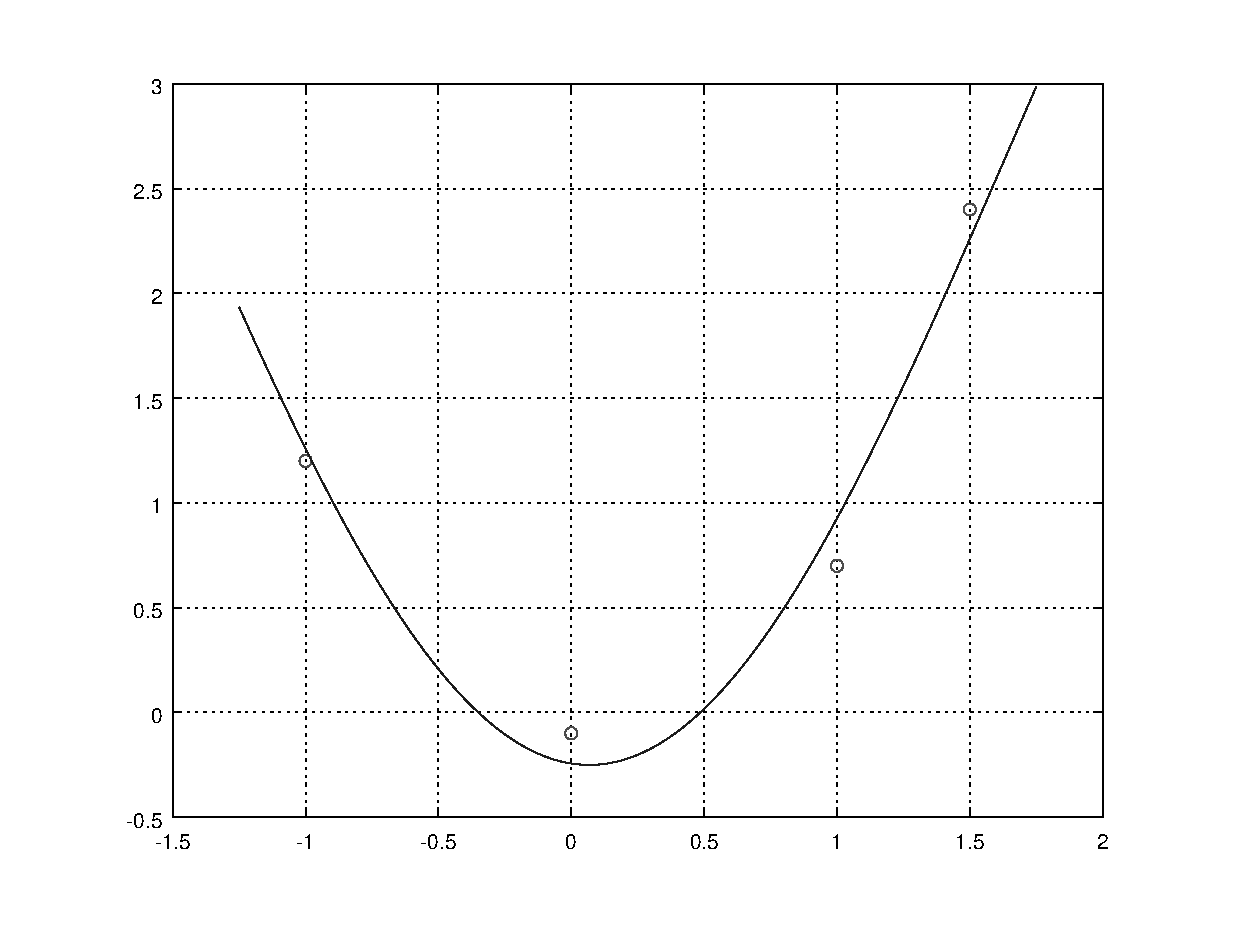
\includegraphics[width=\textwidth]{cap_ajuste/dados/ex_mq_curvas/ex_mq_curvas}
    \caption{Esboço da curva ajustada no Exemplo~\ref{ex:ajuste_de_curvas}.}
    \label{fig:ex_mq_poli}
  \end{figure}

\ifisoctave
Os coeficientes e um esboço do polinômio ajustado podem ser obtidos no \verb+GNU Octave+ com o seguinte código:
\begin{verbatim}
#pontos
x = [-1 0 1 1.5]';
y = [1.2, -0.1, 0.7, 2.4]';

#resol. as eqs. normais
A = [sin(x) cos(x) ones(4,1)];
c = inv(A'*A)*A'*y

#curva ajustada
f = @(x) c(1)*sin(x) + c(2)*cos(x) + c(3)

#esboco da fun. ajustada
xx = linspace(-1.25,1.75);
plot(x,y,'ro',...
     xx,f(xx));grid
\end{verbatim}
\fi

\end{ex}

\begin{ex}\normalfont{(Um problema não linear)}\label{ex:mq_nlin0}
  Consideremos o problema de ajustar, no sentido de mínimos quadrados, à função
  \begin{equation}
    f(x) = c_1e^{c_2x}
  \end{equation}
ao seguinte conjunto de pontos
\begin{center}
  \begin{tabular}{l|rrrr}
    $i$ & $1$ & $2$ & $3$ & $4$ \\\hline
    $x_i$ & $-1$ & $0$ & $1$ & $1,5$\\
    $y_i$ & $8,0$ & $1,5$ & $0,2$ & $0,1$\\\hline
  \end{tabular}
\end{center}

Aqui, temos um problema não linear de mínimos quadrados que pode ser transformado em um problema linear fazendo-se
\begin{align}
  y = c_1e^{c_2x} &\Rightarrow \ln y = \ln c_1e^{c_2x}\\
                  &\Rightarrow \ln y = \ln c_1 + c_2x.
\end{align}
Isto é, denotando $d_1 := \ln c_1$ e $d_2 := c_2$, o problema se resume a ajustar uma reta $r(x) = d_1 + d_2x$ ao conjunto de pontos $\{(x_i, \ln y_i)\}_{i=1}^4$. 

Para resolver o problema transformado, formamos a matriz
\begin{equation}
  A :=
  \begin{bmatrix}
    1 & x_1 \\
    1 & x_2 \\
    1 & x_3 \\
    1 & x_4
  \end{bmatrix}
\end{equation}
e, então, resolvemos as equações normais $A^TAd = A^T\ln y$, com $\ln y = (\ln y_1, \ln y_2, \ln y_3, \ln y_4)$, donde obtemos $d_1=0,315$ e $d_2=-1,792$. Das definições de $d_1$ e $d_2$, temos $c_2 = d_2 = -1,792$ e $c_1 = e^{d_1} = 1,371$. A Figura~\ref{fig:ex_mq_nlin0} mostra um esboço da curva $f(x) = c_1e^{c_2x}$ ajustada (linha azul) aos pontos dados (círculos vermelhos).

\begin{figure}[h]
  \centering
  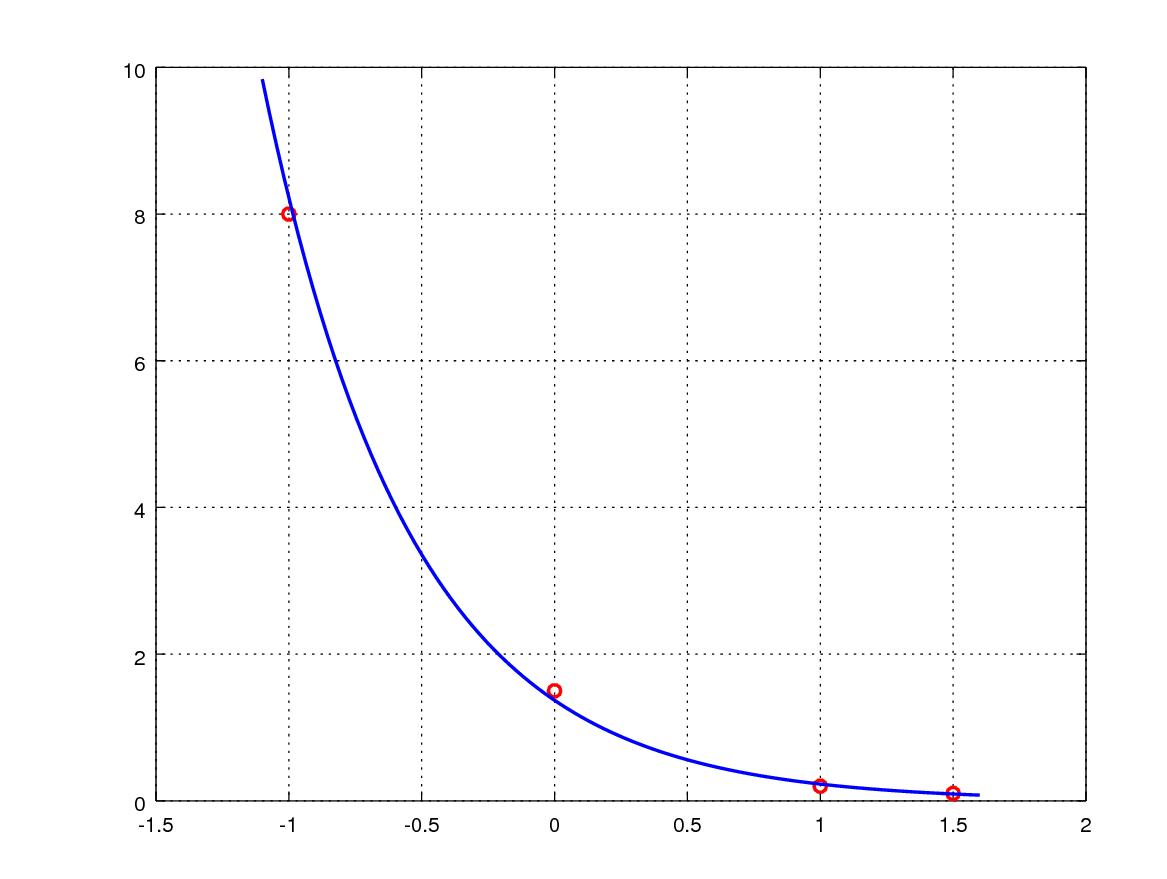
\includegraphics[width=\textwidth]{cap_ajuste/dados/ex_mq_nlin0/ex_mq_nlin0}
  \caption{Esboço da curva ajustada no Exemplo~\ref{ex:mq_nlin0}.}
  \label{fig:ex_mq_nlin0}
\end{figure}

\ifisoctave
O ajuste e um esboço da função ajustada podem ser feitos no \verb+GNU Octave+ com o seguinte código:
\begin{verbatim}
#pontos
x = [-1 0 1 1.5]';
y = [8.0 1.5 0.2 0.1]';

#resol. as eqs. normais
A = [ones(4,1) x];
d = inv(A'*A)*A'*log(y)

#fun. ajustada
c = [exp(d(1)); d(2)]
f = @(x) c(1)*exp(c(2)*x);

#esboco da fun. ajustada
xx = linspace(-1.1,1.6);
plot(x,y,'ro','linewidth',1.5,...
     xx,f(xx),'b-','linewidth',1.5);grid
\end{verbatim}
\fi

\end{ex}

\subsection*{Exercícios}

\begin{exer}\label{exer:mq_reta}
  Determine a reta $y = c_1x + c_2$ que melhor se ajusta, no sentido de mínimos quadrados, aos pontos
  \begin{center}
    \begin{tabular}{l|ccccc}
      $i$ & $1$ & $2$ & $3$ & $4$ & $5$ \\\hline
      $x_i$ & $-2,5$ & $-1,3$ & $0,2$ & $1,7$ & $2,3$\\
      $y_i$ & $3,8$ & $1,5$ & $-0,7$ & $-1,5$ & $-3,2$\\\hline
    \end{tabular}
  \end{center}
Por fim, compute a norma $L^2$ do resíduo, i.e. $\|r(c)\|_2 = \|y - (c_1x - c_2)\|_2$ para os pontos dados.
\end{exer}
\begin{resp}
  $c_1 = -1,3259$, $c_2 = 8,66071\E-2$, $\|r(c)\|_2 = 1,01390$.
\end{resp}

\begin{exer}\label{exer:mq_poli}
  Determine o polinômio $y = c_1x^3 + c_2x^2 + c_3x + c_4$ que melhor se ajusta, no sentido de mínimos quadrados, aos pontos
  \begin{center}
    \begin{tabular}{l|ccccc}
      $i$ & $1$ & $2$ & $3$ & $4$ & $5$ \\\hline
      $x_i$ & $-2,5$ & $-1,3$ & $0,2$ & $1,7$ & $2,3$\\
      $y_i$ & $3,8$ & $0,5$ & $2,7$ & $1,2$ & $-1,3$\\\hline
    \end{tabular}
  \end{center}
Por fim, compute a norma $L^2$ do resíduo, i.e. $\|r(c)\|_2$.
\end{exer}
\begin{resp}
  $c_1 = -4,50361\E-1$, $c_2 = -2,78350\E-1$, $c_3 = 1,46291$, $c_4 = 2,09648$, $\|r(c)\|_2 = 5,71346$
\end{resp}

\begin{exer}\label{exer:mq_curva}
  Determine a curva $y = c_1\sen x + c_2\cos x + c_3$ que melhor se ajusta, no sentido de mínimos quadrados, aos pontos
  \begin{center}
    \begin{tabular}{l|ccccc}
      $i$ & $1$ & $2$ & $3$ & $4$ & $5$ \\\hline
      $x_i$ & $-2,5$ & $-1,3$ & $0,2$ & $1,7$ & $2,3$\\
      $y_i$ & $3,8$ & $0,5$ & $2,7$ & $1,2$ & $-1,3$\\\hline
    \end{tabular}
  \end{center}
Por fim, compute a norma $L^2$ do resíduo, i.e. $\|r(c)\|_2$.
\end{exer}
\begin{resp}
  $c_1 = -2,76842$, $c_2 = -7,17935\E-1$, $c_3 = 1,37014\E-1$, $\|r(c)\|_2 = 2,48880\E+1$
\end{resp}

\begin{exer}\label{exer:mq_nlin0}
  Use a transformação $z = \ln y$ para ajustar, no sentido de mínimos quadrados, a curva $y = c_1e^{c_2(x-c_3)^2}$ aos pontos
  \begin{center}
    \begin{tabular}{l|cccccc}
      $i$ & $1$ & $2$ & $3$ & $4$ & $5$ & $6$ \\\hline
      $x_i$ & $-0,5$ & $0,5$ & $1,3$ & $2,1$ & $2,7$ & $3,1$ \\
      $y_i$ & $0,1$ & $1,2$ & $2,7$ & $0,9$ & $0,2$ & $0,1$ \\\hline
    \end{tabular}
  \end{center}
\end{exer}
\begin{resp}
  $c_1 = 2,10131\E+0$, $c_2 = -9,73859\E-1$, $c_3 = 1.25521\E+0$
\end{resp}
   
\section{Problemas não lineares}\label{cap_ajuste_sec_prob_nlin}

Um problema não linear de mínimos quadrados consiste em ajustar uma dada função $f(x;c)$ que dependa não linearmente dos parâmetros $c = (c_1, c_2, \dotsc, c_m)$, $m\geq 1$, a um dado conjunto de $n\geq m$ pontos $\{(x_i, y_i)\}_{i=1}^n$. Mais especificamente, buscamos resolver o seguinte problema de minimização
\begin{equation}\label{eq:prob_nlin_mq}
  \min_{\{c_1, c_2, \dotsc, c_m\}} \left[E := \sum_{i=1}^n \left(y_i - f(x_i;c)\right)^2\right].
\end{equation}
Aqui, denotaremos por $r(c) := (r_1(c), r_2(c), \dotsc, r_n(c))$ o vetor dos resíduos $r_i(c) := y_i - f(x_i,c)$. Com isso, o problema se resume a encontrar o vetor de parâmetros $c$ que minimiza
\begin{equation}
  E = \|r(c)\|_2^2.
\end{equation}
Tais parâmetros são solução do seguinte sistema de equações
\begin{equation}
  \frac{\p E}{\p c_j} = 2\sum_{i=1}^n r_i(c)\frac{\p}{\p c_j}r_i(c)
\end{equation}
ou, equivalentemente, da equação
\begin{equation}\label{eq:grad_E}
  \nabla E = 0 \Leftrightarrow J_R^T(c)r(c) = 0,
\end{equation}
onde
\begin{equation}
  J_R(c) :=
  \begin{bmatrix}
    \frac{\p r_1}{\p c_1} & \frac{\p r_1}{\p c_2} & \cdots & \frac{\p r_1}{\p c_m}\\
    \frac{\p r_2}{\p c_1} & \frac{\p r_2}{\p c_2} & \cdots & \frac{\p r_2}{\p c_m}\\
    \vdots  & \vdots & \vdots & \vdots \\
    \frac{\p r_n}{\p c_1} & \frac{\p r_n}{\p c_2} & \cdots & \frac{\p r_n}{\p c_m}
  \end{bmatrix}
\end{equation}
é a jacobiana do resíduo $r$ em relação aos parâmetros $c$.

Podemos usar o método de Newton para resolver~\eqref{eq:grad_E}. Para tanto, escolhemos uma aproximação inicial para $c^{(1)} = (c_1^{(1)}, c_2^{(1)}, \dotsc, c_m^{(1)})$ e iteramos
\begin{align}
  H_R(c^{(k)})\delta^{(k)} &= -J_R^T(c)r(c) \label{eq:mqnl_newton1}\\
  c^{(k+1)} &= c^{(k)} + \delta^{(k)} \label{eq:mqnl_newton2},
\end{align}
onde $\delta^{(k)} = (\delta_1^{(k)}, \delta_2^{(k)}, \delta_m^{(k)})$ é a atualização de Newton (ou direção de busca) e $H_R(c) := [h_{p,q}(c)]_{p,q=1}^{m,m}$ é a matriz hessiana, cujos elementos são
\begin{equation}
  h_{p,q} := \sum_{i=1}^n\left\{\frac{\p r_i}{\p c_q}\frac{\p r_i}{\p c_p} + r_i\frac{\p^2 r_i}{\p c_q\p c_p}\right\}.
\end{equation}

\begin{ex}\label{ex:mqnl_newton}
  Consideremos o problema de ajustar, no sentido de mínimos quadrados, a função
  \begin{equation}
    f(x;c) = c_1e^{c_2x}
  \end{equation}
ao seguinte conjunto de pontos
\begin{center}
  \begin{tabular}{l|rrrr}
    $i$ & $1$ & $2$ & $3$ & $4$ \\\hline
    $x_i$ & $-1$ & $0$ & $1$ & $1,5$\\
    $y_i$ & $8,0$ & $1,5$ & $0,2$ & $0,1$\\\hline
  \end{tabular}
\end{center}

Aqui, vamos utilizar a iteração de Newton para o problema de mínimos quadrados, i.e. a iteração dada em \eqref{eq:mqnl_newton1}-\eqref{eq:mqnl_newton2}. Para tanto, para cada $i=1, 2, 3, 4$, precisamos das seguintes derivadas parciais do resíduo $r_i(c) := y_i - c_1e^{c_2x_i}$:
\begin{align}
  &\frac{\p}{\p c_1}r_i(c) = - e^{c_2x_i},\\
  &\frac{\p}{\p c_2}r_i(c) = - c_1x_ie^{c_2x_i},\\
  &\frac{\p^2}{\p c_1^2}r_i(c) = 0,\\
  &\frac{\p^2}{\p c_1\p c_2}r_i(c) = \frac{\p^2}{\p c_2\p c_1}r_i(c) = - x_ie^{c_2x_i},\\
  &\frac{\p^2}{\p c_2^2}r_i(c) = - c_1x_i^2e^{c_2x_i}.
\end{align}

\begin{figure}[h]
  \centering
  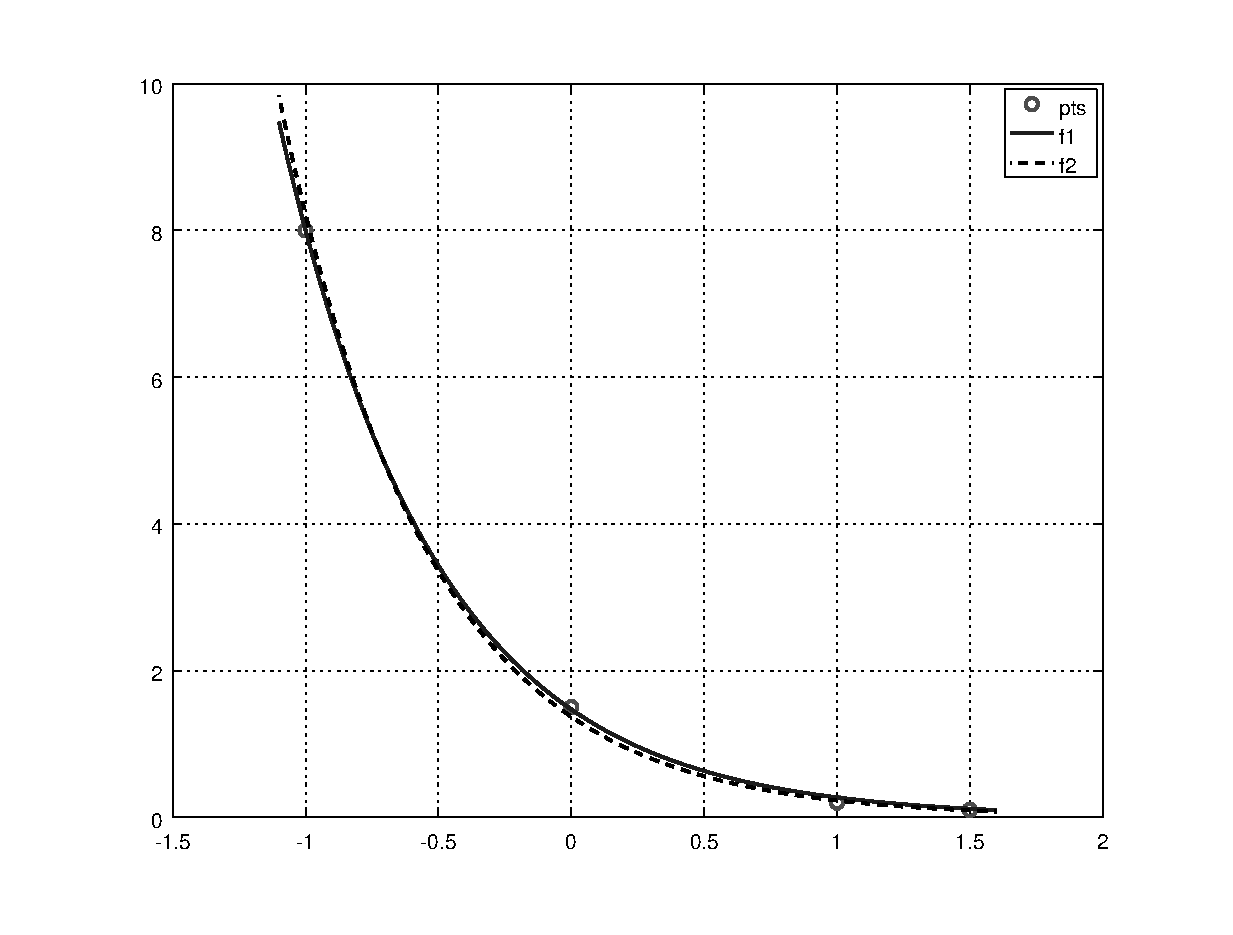
\includegraphics[width=\textwidth]{cap_ajuste/dados/ex_mqnl_N/ex_mqnl_N}
  \caption{Esboço da curva ajustada no Exemplo~\ref{ex:mqnl_newton}.}
  \label{fig:ex_mqnl_newton}
\end{figure}

Com isso e tomando $c^{(1)} = (1,4, ~-1,8)$ (motivado do Exemplo~\ref{ex:mq_nlin0}), computamos as iterações de Newton~\eqref{eq:mqnl_newton1}-\eqref{eq:mqnl_newton2}. Iterando até a precisão de $TOL = 10^{-4}$, obtemos a solução $c_1 = 1,471$ e $c_2 = -1,6938$. Na Figura~\ref{fig:ex_mqnl_newton} vemos uma comparação entre a curva aqui ajustada ($-$) e aquela obtida no Exemplo~\ref{ex:mq_nlin0} ($--$).

\ifisoctave
O ajuste discutido neste exemplo pode ser computado no \verb+GNU Octave+ com o seguinte código:
\begin{verbatim}
#pontos
global x = [-1 0 1 1.5]';
global y = [8.0 1.5 0.2 0.1]';

#fun. objetivo
f = @(x,c) c(1)*exp(c(2)*x);

#residuo
r = @(c) y - f(x,c);

#jacobiana
function A = J(c)
  global x
  A = zeros(4,2);
  A(:,1) = - exp(c(2)*x);
  A(:,2) = - c(1)*x.*exp(c(2)*x);
endfunction

#hessiana
function A = H(c)
  global x
  global y
  A = zeros(2,2);
  A = J(c)'*J(c);
  for i=1:4
    A(1,1) += 0;
    A(1,2) += (y(i) - c(1)*exp(c(2)*x(i))) * ...
              (- x(i)*exp(c(2)*x(i)));
    A(2,1) += (y(i) - c(1)*exp(c(2)*x(i))) * ...
              (- x(i)*exp(c(2)*x(i)));
    A(2,2) += (y(i) - c(1)*exp(c(2)*x(i))) * ...
              (- c(1)*x(i)^2*exp(c(2)*x(i)));
  endfor
endfunction

#aprox. inicial
c = [1.4 -1.8]';

#iteracoes de Newton
k=0;
do
  k+=1;
  delta = - inv(H(c))*J(c)'*r(c);
  c = c + delta;
  [k,c',norm(delta)]
until ((k>10) | (norm(delta)<1e-4))
\end{verbatim}
\fi
\end{ex}

Observamos que a solução obtida no exemplo anterior (Exemplo~\ref{ex:mqnl_newton}) difere da previamente encontrada no Exemplo~\ref{ex:mq_nlin0}. Naquele exemplo, os parâmetros obtidos nos fornecem $E = 6,8\E-2$, enquanto que a solução do exemplo anterior fornece $E = 6,1\E-3$. Isto é esperado, pois naquele exemplo resolvemos um problema aproximado, enquanto no exemplo anterior resolvemos o problema por si.

O emprego do método de Newton para o problema de mínimos quadrados tem a vantagem da taxa de convergência quadrática, entretanto requer a computação das derivadas parciais de segunda ordem do resíduo. Na sequência discutimos alternativas comumente empregadas.

\subsection{Método de Gauss-Newton}

O método de Gauss-Newton é uma técnica iterativa que aproxima o problema não linear de mínimos quadrados \eqref{eq:prob_nlin_mq} por uma sequência de problemas lineares. Para seu desenvolvimento, começamos de uma aproximação inicial $c^{(1)} = (c_1^{(1)}, c_2^{(1)}, \dotsc, c_m^{(1)})$ dos parâmetros que queremos ajustar. Também, assumindo que a $n$-ésima iterada $c^{(k)}$ é conhecida, faremos uso da aproximação de primeira ordem de $f(x,c)$ por polinômio de Taylor, i.e.
\begin{equation}
  f(x;c^{(k+1)}) \approx f(x;c^{(k)}) + \nabla_c f(x;c^{(k)})(c^{(k+1)}-c^{(k)}),
\end{equation}
onde
\begin{equation}
  \nabla_c f(x;c) = \left[\frac{\p}{\p c_1}f(x;c) ~\frac{\p}{\p c_2}f(x;c) ~\cdots ~\frac{\p}{\p c_m}f(x;c)\right].
\end{equation}

O método consiste em obter a solução do problema não linear \eqref{eq:prob_nlin_mq} pelo limite dos seguintes problemas lineares de mínimos quadrados
\begin{align}
  \min_{\delta^{(k)}} &\left[\tilde{E} := \sum_{i=1}^n (y_i - f(x_i,c^{(k)}) - \nabla_c f(x_i;c^{(k)})\delta^{(k)})^2\right] \label{eq:mq_gn0}\\
  &c^{(k+1)} = c^{(k)} + \delta^{(k)}.
\end{align}

Agora, usando a notação de resíduo $r(c) = y - f(x;c)$, observamos que \eqref{eq:mq_gn0} consiste no problema linear de mínimos quadrados
\begin{equation}
  \min_{\delta^{(k)}} \|r(c^{(k)}) + J_R(c^{(k)})\delta^{(k)}\|_2^2,
\end{equation}
o qual é equivalente a resolver as equações normais
\begin{equation}
  J_R^T(c^{(n)})J_R(c^{(n)})\delta^{(n)} = -J_R^T(c)r(c).
\end{equation}

Com isso, dada uma aproximação inicial $c^{(1)}$, a \emph{iteração do método de Gauss-Newton} consiste em
\begin{align}
  &J_R^T(c^{(k)})J_R(c^{(k)})\delta^{(k)} = -J_R^T(c)r(c)\\
  &c^{(k+1)} = c^{(k)} + \delta^{(k)}.
\end{align}

\begin{ex}
  A aplicação da iteração de Gauss-Newton ao problema de mínimos quadrados discutido no Exemplo~\ref{ex:mqnl_newton} nos fornece a mesma solução obtida naquele exemplo (preservadas a aproximação inicial e a tolerância de precisão).

\ifisoctave
A implementação do método de Gauss-Newton para este problema no \verb+GNU Octave+ pode ser feita com o seguinte código:
\begin{verbatim}
#pontos
global x = [-1 0 1 1.5]';
y = [8.0 1.5 0.2 0.1]';

#fun. objetivo
f = @(x,c) c(1)*exp(c(2)*x);

#residuo
r = @(c) y - f(x,c);

#jacobiana
function A = J(c)
  global x
  A = zeros(4,2);
  A(:,1) = - exp(c(2)*x);
  A(:,2) = - c(1)*x.*exp(c(2)*x);
endfunction

#aprox. inicial
c = [1.4 -1.8]';

#iteracoes de Gauss-Newton
k=0;
do
  k+=1;
  delta = - inv(J(c)'*J(c))*J(c)'*r(c);
  c = c + delta;
  [k,c',norm(delta)]
until ((k>10) | (norm(delta)<1e-4))
\end{verbatim}
\fi
\end{ex}

O método de Gauss-Newton pode ser lentamente convergente para problemas muito não lineares ou com resíduos grandes. Nesse caso, métodos de Gauss-Newton com amortecimento são alternativas robustas~\cite{Bjorck1996a,Nocedal2006a}. Na sequência, introduziremos um destes métodos, conhecido como método de Levenberg-Marquardt.

\subsection{Método de Levenberg-Marquardt}

O método de Levenberg-Marquardt é uma variação do método de Gauss-Newton no qual a direção de busca $\delta^{(n)}$ é obtida da solução do seguinte problema regularizado
\begin{equation} \label{eq:mq_gn0}
  \min_{\delta^{(k)}} \{\|r(c^{(k)}) + J_R(c^{(k)})\delta^{(k)}\|_2^2 + \mu^{(k)}\|\delta^{(k)}\|_2^2\}
\end{equation}
ou, equivalentemente,
\begin{equation} \label{eq:mq_gn0}
  \min_{\delta^{(k)}} \left\|
    \begin{bmatrix}
      r(c^{(k)})\\
      0
    \end{bmatrix} +
    \begin{bmatrix}
      J_R(c^{(k)})\\
      \mu^{(k)}I
    \end{bmatrix}
    \delta^{(k)}\right\|_2^2
\end{equation}

A taxa de convergência das iterações de Levenberg-Marquardt é sensível a escolha do parâmetro $\mu^{(k)}\geq 0$. Aqui, faremos esta escolha por tentativa e erro. O leitor pode aprofundar-se mais sobre esta questão na literatura especializada (veja, por exemplo, \cite{Bjorck1996a,Nocedal2006a}).

\begin{obs}
  Quando $\mu^{(k)} \equiv 0$ para todo $n$, o método de Levenberg-Marquardt é equivalente ao método de Gauss-Newton.
\end{obs}

\begin{ex}\label{ex:mqnl_LM}
  Consideremos o problema de mínimos quadrados discutido no Exemplo~\ref{ex:mqnl_newton}. O método de Gauss-Newton falha para este problema se escolhermos, por exemplo, $c^{(1)} = (0, 0)$. Isto ocorre pois, para esta escolha de $c^{(1)}$, a jacobiana $J(c^{(1)})$ não tem posto completo. Entretanto, o método de Levenberg-Marquardt com $\mu^{(k)} = 0,1$ é convergente, mesmo para esta escolha de $c^{(1)}$.

\ifisoctave
A implementação no \verb+GNU Octave+ do método de Levenberg-Marquardt (com $\mu^{(k)}=0,1$ constante) para este problema pode ser feita com o seguinte código:
\begin{verbatim}
#pontos
global x = [-1 0 1 1.5]';
y = [8.0 1.5 0.2 0.1]';

#fun. objetivo
f = @(x,c) c(1)*exp(c(2)*x);

#residuo
r = @(c) y - f(x,c);

#jacobiana
function A = JR(c)
  global x;
  A = zeros(4,2);
  A(:,1) = - exp(c(2)*x);
  A(:,2) = - c(1)*x.*exp(c(2)*x);
endfunction

#aprox. inicial
c = [0 0]';

#param. de amortecimento
mu = 0.1;

#iteracoes de Gauss-Newton
k=0;
do
  k+=1;
  JJ = [JR(c);mu*eye(2,2)];
  delta = - inv(JJ'*JJ)*JJ'*[r(c);zeros(2,1)];
  c = c + delta;
  printf("%d %1.1e %1.3e %1.3e\n", k,norm(delta),c')
until ((k>10) | (norm(delta)<1e-4))
\end{verbatim}
\fi
\end{ex}

\subsection*{Exercícios}

\begin{exer}\label{exer:mqnl_GN}
  Use o método de Gauss-Newton para ajustar, no sentido de mínimos quadrados e com precisão de $10^{-4}$, a curva $y = c_1e^{c_2(x-c_3)^2}$ aos pontos
  \begin{center}
    \begin{tabular}{l|cccccc}
      $i$ & $1$ & $2$ & $3$ & $4$ & $5$ & $6$ \\\hline
      $x_i$ & $-0,5$ & $0,5$ & $1,3$ & $2,1$ & $2,7$ & $3,1$ \\
      $y_i$ & $0,1$ & $1,2$ & $2,7$ & $0,9$ & $0,2$ & $0,1$ \\\hline
    \end{tabular}
  \end{center}
Use as condições iniciais:
\begin{enumerate}[a)]
\item $c_1 = 2,1$, $c_2=-1$ e $c_3=1,3$.
\item $c_1=1$, $c_2=-1$ e $c_3=-1$.
\end{enumerate}
\end{exer}
\begin{resp}
  a) $c_1 = 2,69971\E+0$, $c_2 = -1,44723\E+0$, $c_3 = 1.24333\E+0$; b) divergente.
\end{resp}

\begin{exer}
  Resolva o exercício anterior (Exercício~\ref{exer:mqnl_GN}) usando o método de Levenberg-Marquardt com amortecimento constante $\mu=0,2$.
\end{exer}
\begin{resp}
  a)  $c_1 = 2,69971\E+0$, $c_2 = -1,44723\E+0$, $c_3 = 1.24333\E+0$; b) $c_1 = 2,69971\E+0$, $c_2 = -1,44723\E+0$, $c_3 = 1.24333\E+0$
\end{resp}

%Este trabalho está licenciado sob a Licença Atribuição-CompartilhaIgual 4.0 Internacional Creative Commons. Para visualizar uma cópia desta licença, visite http://creativecommons.org/licenses/by-sa/4.0/deed.pt_BR ou mande uma carta para Creative Commons, PO Box 1866, Mountain View, CA 94042, USA.

\chapter{Derivação}\label{cap_deriv}
\thispagestyle{fancy}

Neste capítulo, discutimos os métodos fundamentais de derivação numérica de funções.

\section{Derivadas de primeira ordem}\label{cap_deriv_sec_df}

A derivada de uma função $f$ num ponto $x$ é, por definição,
\begin{equation}
  f'(x) = \lim_{h\to 0} \frac{f(x+h) - f(x)}{h}.
\end{equation}
Assim sendo e assumindo $h>0$\footnote{Para fixar notação, assumiremos $h>0$ ao longo deste capítulo.} próximo de zero, temos que $f'(x)$ pode ser aproximada pela razão fundamental, i.e.
\begin{equation}\label{eq_razao_fundamental}
  f'(x) \approx \underbrace{\frac{f(x+h) - f(x)}{h}}_{D_hf(x)}.
\end{equation}
Analisando a Figura~\ref{fig:intro_deriv} vemos que, geometricamente, isto é análogo a aproximar a declividade da reta tangente ao gráfico da função $f$ no ponto $(x,f(x))$ pela declividade da reta secante ao gráfico da função $f$ pelos pontos $(x,f(x))$ e $(x+h,f(x+h))$.

\begin{figure}[hp]
  \centering
  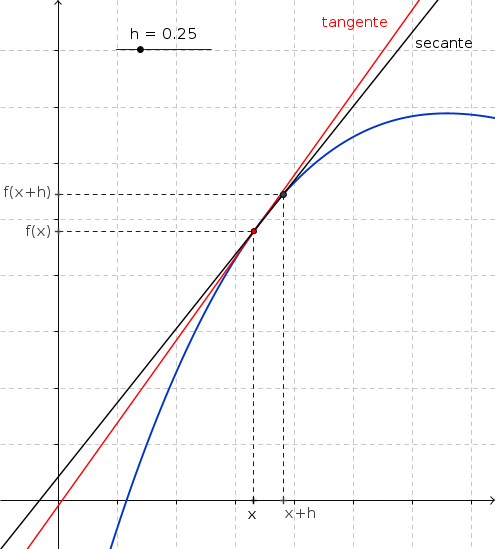
\includegraphics[width=0.7\textwidth]{cap_deriv/dados/fig_intro_deriv/fig_intro_deriv}
  \caption{Interpretação geométrica da aproximação da derivada pela razão fundamental. Veja no \href{https://github.com/phkonzen/notas/blob/master/src/MatematicaNumerica/cap_deriv/dados/fig_intro_deriv/fig_intro_deriv.ggb}{Geogebra}.}
  \label{fig:intro_deriv}
\end{figure}

\begin{ex}\label{ex_intro_deriv}
  A derivada de $f(x) = \sen(x)$ no ponto $\pi/3$ é $f'(\pi/3) = \cos(\pi/3)=0,5$. Agora, usando a aproximação pela razão fundamental~\eqref{eq_razao_fundamental}, temos
  \begin{align}
    f'\left(\frac{\pi}{3}\right) \approx D_hf(x) &= \frac{f\left(\frac{\pi}{3}+h\right)-f\left(\frac{\pi}{3}\right)}{h}\\
          &= \frac{\sen\left(\frac{\pi}{3}\right)-\sen\left(\frac{\pi}{3}\right)}{h}. 
  \end{align}
Na Tabela~\ref{tab:ex_intro_deriv} temos os valores desta aproximação para diferentes escolhas da passo $h$.

\begin{table}[hp]
  \centering
  \begin{tabular}{l|c}
    $h$ & $Df(\pi/3)$ \\ \hline
    $10^{-1}$ & $4,55902\E-1$ \\
    $10^{-2}$ & $4,95662\E-1$ \\
    $10^{-3}$ & $4,99567\E-1$ \\
    $10^{-5}$ & $4,99996\E-1$ \\
    $10^{-10}$ & $5.00000\E-1$ \\\hline
  \end{tabular}
  \caption{Valores aproximados da derivada de $f(x)=\sen(x)$ no ponto $x=\pi/6$ usado a expressão~\eqref{eq_razao_fundamental}.}
  \label{tab:ex_intro_deriv}
\end{table}
\end{ex}

A aproximação~\eqref{eq_razao_fundamental} é uma \emph{fórmula de diferenças finitas}\index{diferenças finitas}. Existem várias aproximações deste tipo que podem ser derivadas. Além disso, tais derivações nos permitem estimar o erro na utilização de tais fórmulas para a aproximação de derivadas. Na sequência, discutiremos o desenvolvimento de fórmulas de diferenças finitas usando polinômios de Taylor.

\subsection{Desenvolvimento por polinômio de Taylor}

Aqui, discutimos a obtenção de fórmulas de diferenças finitas via polinômio de Taylor.

\subsubsection{Diferenças finitas progressiva de ordem $h$}

A aproximação por polinômio de Taylor de grau 1 de uma dada função $f$ em torno no ponto $x$ é
\begin{equation}\label{eq:poli_Taylor_grau_1}
  f(x+h) = f(x) + hf'(x) + O(h^2).
\end{equation}
Agora, isolando $f'(x)$, obtemos
\begin{equation}
  f'(x) = \frac{f(x+h) - f(x)}{h} + O(h).
\end{equation}
Isto nos fornece a chamada fórmula de diferenças finitas progressiva de ordem $h$\index{diferenças finitas!progressiva de ordem $h$}
\begin{equation}\label{eq:dfp_h}
  D_{+,h}f(x) := \frac{f(x+h) - f(x)}{h}.
\end{equation}
Observemos que a ordem da fórmula se refere a ordem do erro de truncamento com respeito ao passo $h$.

\begin{ex}\label{ex:dfp_h}
  Consideremos o problema de aproximar a derivada da função $f(x) = \sen(x)$ no ponto $\pi/3$. Usando a fórmula de diferenças finitas progressiva de ordem $h$ obtemos
  \begin{align}
    f'\left(\frac{\pi}{3}\right) \approx D_{+,h}f(x) &= \frac{f\left(\frac{\pi}{3}+h\right)-f\left(\frac{\pi}{3}\right)}{h}\\
          &= \frac{\sen\left(\frac{\pi}{3}+h\right)-\sen\left(\frac{\pi}{3}\right)}{h}. 
  \end{align}
Na Tabela~\ref{tab:ex_dfp_h} temos os valores desta aproximação para diferentes escolhas de $h$, bem como, o erro absoluto da aproximação de $f'(\pi/3)$ por $D_{+,h}f(\pi/3)$.

\begin{table}[h!]
  \centering
  \caption{Resultados referente ao Exemplo~\ref{ex:dfp_h}.}
  \begin{tabular}{l|c|c}
    $h$ & $D_{+,h}f(\pi/3)$ & $|f'(\pi/3)-D_{+,h}f(\pi/3)|$\\ \hline
    $10^{-1}$ & $4,55902\E-1$ & $4,4\E-2$ \\
    $10^{-2}$ & $4,95662\E-1$ & $4,3\E-3$ \\
    $10^{-3}$ & $4,99567\E-1$ & $4,3\E-4$ \\
    $10^{-5}$ & $4,99996\E-1$ & $4,3\E-6$ \\
    $10^{-10}$ & $5.00000\E-1$ & $4,1\E-8$ \\\hline
  \end{tabular}
  \label{tab:ex_dfp_h}
\end{table}
\end{ex}

\begin{obs}
  No exemplo acima (Exemplo~\ref{ex:dfp_h}), podemos observar que o erro absoluto na aproximação de $f'(x)$ por $D_{+,h}f(x)$ decresce conforme a ordem do erro de truncamento para valores moderados de $h$ (veja, Tabela~\ref{tab:ex_dfp_h}). Agora, para valores de $h$ muito pequenos (por exemplo, $h=10^{-10}$), o erro $|f'(x)-D_{+,h}f(x)|$ não segue mais a tendência de decaimento na mesma do de truncamento. Isto se deve a dominância dos erros de arredondamento para valores muito pequenos de $h$. 

  Para mais informações sobre o comportamento do erro de arredondamento em fórmulas de diferenças finitas, veja, por exemplo, \href{https://www.ufrgs.br/reamat/CalculoNumerico/livro-oct/dn-diferencas_finitas.html}{REAMAT - Cálculo Numérico - Versão GNU Octave - Diferenças Finitas - Erro de arredondamento}.
\end{obs}

\subsubsection{Diferenças finitas regressiva de ordem $h$}

Substituindo $h$ por $-h$ na equação~\eqref{eq:poli_Taylor_grau_1}, obtemos
\begin{equation}
  f(x-h) = f(x) - hf'(x) + O(h^2),
\end{equation}
donde obtemos a fórmula de diferenças finitas regressiva de ordem $h$\index{diferenças finitas!regressiva de ordem $h$}
\begin{equation}\label{eq:dfr_h}
  D_{-,h}f(x) = \frac{f(x) - f(x-h)}{h}.
\end{equation}

\begin{ex}\label{ex:dfr_h}
  Consideremos o problema de aproximar a derivada da função $f(x) = \sen(x)$ no ponto $\pi/3$. Usando a fórmula de diferenças finitas regressiva de ordem $h$ obtemos
  \begin{align}
    f'\left(\frac{\pi}{3}\right) \approx D_{-,h}f(x) &= \frac{f\left(\frac{\pi}{3}\right)-f\left(\frac{\pi}{3}-h\right)}{h}\\
          &= \frac{\sen\left(\frac{\pi}{3}\right)-\sen\left(\frac{\pi}{3}-h\right)}{h}. 
  \end{align}
Na Tabela~\ref{tab:ex_dfr_h} temos os valores desta aproximação para diferentes escolhas de $h$, bem como, o erro absoluto da aproximação de $f'(\pi/3)$ por $D_{-,h}f(\pi/3)$.

\begin{table}[h!]
  \centering
  \caption{Resultados referente ao Exemplo~\ref{ex:dfr_h}.}
  \begin{tabular}{l|c|c}
    $h$ & $D_{-,h}f(\pi/3)$ & $|f'(\pi/3)-D_{-,h}f(\pi/3)|$\\ \hline
    $10^{-1}$ & $5,42432\E-1$ & $4,2\E-2$ \\
    $10^{-2}$ & $5,04322\E-1$ & $4,3\E-3$ \\
    $10^{-3}$ & $5,00433\E-1$ & $4,3\E-4$ \\
    $10^{-5}$ & $5,00004\E-1$ & $4,3\E-6$ \\
    $10^{-10}$ & $5.00000\E-1$ & $4,1\E-8$ \\\hline
  \end{tabular}
  \label{tab:ex_dfr_h}
\end{table}
\end{ex}

\subsubsection{Diferenças finitas central de ordem $h^2$}

Usando o polinômio de Taylor de grau 2 para aproximar a função $f(x)$ em torno de $x$, obtemos
\begin{align}
  f(x+h) &= f(x) + hf'(x) + \frac{h}{2}f''(x) + O(h^3)\\
  f(x-h) &= f(x) - hf'(x) + \frac{h}{2}f''(x) + O(h^3).
\end{align}
Então, subtraindo esta segunda equação da primeira, temos
\begin{equation}
  f(x+h)-f(x-h) = 2hf(x) + O(h^3).
\end{equation}
Agora, isolando $f(x)$
\begin{equation}
  f(x) = \frac{f(x+h)-f(x-h)}{2h} + O(h^2),
\end{equation}
o que nos fornece a chamada fórmula de diferenças finitas central de ordem $h^2$\index{diferenças finitas!central de ordem $h^2$}
\begin{equation}\label{eq:dfc_h2}
  D_{0,h^2}f(x) := \frac{f(x+h)-f(x-h)}{2h}.
\end{equation}

\begin{ex}\label{ex:dfc_h2}
  Consideremos o problema de aproximar a derivada da função $f(x) = \sen(x)$ no ponto $\pi/3$. Usando a fórmula de diferenças finitas central de ordem $h^2$ obtemos
  \begin{align}
    f'\left(\frac{\pi}{3}\right) \approx D_{0,h^2}f(x) &= \frac{f\left(\frac{\pi}{3}+h\right)-f\left(\frac{\pi}{3}-h\right)}{2h}\\
          &= \frac{\sen\left(\frac{\pi}{3}+h\right)-\sen\left(\frac{\pi}{3}-h\right)}{2h}. 
  \end{align}

\begin{table}[h!]
  \centering
  \caption{Resultados referente ao Exemplo~\ref{ex:dfc_h2}.}
  \begin{tabular}{l|c|c}
    $h$ & $D_{0,h}f(\pi/3)$ & $|f'(\pi/3)-D_{0,h^2}f(\pi/3)|$\\ \hline
    $10^{-1}$ & $4,99167\E-1$ & $8,3\E-04$ \\
    $10^{-2}$ & $4,99992\E-1$ & $8,3\E-06$ \\
    $10^{-3}$ & $5,00000\E-1$ & $8,3\E-08$ \\
    $10^{-5}$ & $5,00000\E-1$ & $8,3\E-10$ \\
    $10^{-10}$ & $5.00000\E-1$ & $7,8\E-12$ \\\hline
  \end{tabular}
  \label{tab:ex_dfc_h2}
\end{table}

Na Tabela~\ref{tab:ex_dfc_h2} temos os valores desta aproximação para diferentes escolhas de $h$, bem como, o erro absoluto da aproximação de $f'(\pi/3)$ por $D_{0,h^2}f(\pi/3)$.

\end{ex}


\subsection*{Exercícios}

\emconstrucao

\section{Diferenças finitas por polinômios interpoladores}\label{cap_deriv_sec_df_pi}

Aqui, discutimos a obtenção de fórmulas de diferenças finitas por polinômios interpoladores. Seja $p(x)$ o polinômio interpolador dos pontos $\{(x_i,f(x_i))\}_{i=1}^{n+1}$ de uma dada função $f(x)$, com $x_1 < x_2 < \cdots < x_{n+1}$. Então, pelo teorema de Lagrange temos
\begin{equation}
  f(x) = p(x) + R_{n+1}(x),
\end{equation}
onde $R(x)$ é o erro na aproximação de $f(x)$ por $p(x)$ e tem a forma
\begin{equation}
  R_{n+1}(x) = \frac{f^{(n+1)}(\xi)}{(n+1)!}\prod_{j=1}^{n+1}(x-x_j).
\end{equation}
onde $\xi = \xi(x)$.

Deste modo, a ideia para obtermos as fórmulas de diferenças é aproximarmos $f'(x)$ por $p'(x)$. Entretanto, isto nos coloca a questão de estimarmos o erro $|f'(x) - p'(x)|$. Por sorte temos os seguinte teorema.

\begin{teo}\label{teo:erro_de_Lagrange_deriv}
  Seja $p(x)$ o polinômio interpolador de uma dada função $f(x)$ pelo pontos $\{(x_i, f(x_i))\}_{i=1}^{n+1}$, com $x_1<x_2<\cdots<x_{n+1}$. Se $f(x)$ é $(n+1)$ continuamente diferenciável, então o resíduo $R_{n+1}^{(k)}(x) = f^{(k)}(x) - p^{(k)}(x)$ é
  \begin{equation}
    R_{n+1}^{(k)} = \frac{f^{(n+1)}(\eta) }{(n+1-k)!}\prod_{j=1}^{n+1-k}(x-\xi_j),
  \end{equation}
onde $\xi_j$ é um ponto tal que $x_j < \xi_j < x_{j+k}$, $j=1, 2, \dotsc, n+1+k$, e $\eta = \eta(x)$ é algum ponto no intervalo de extremos $x$ e $\xi_j$. 
\end{teo}
\begin{dem}
  Veja \cite[Ch.6, Sec.5]{Isaacson1994a}.
\end{dem}

\subsection{Fórmulas de dois pontos}

Seja $p(x)$ o polinômio interpolador de Lagrange de $f(x)$ pelos pontos $(x_1, f(x_1))$ e $(x_2, f(x_2))$, com $x_1 < x_2$, i.e.
\begin{align}
  f(x) &= p(x) + R_{2}(x)\\
  &= f(x_1)\frac{x-x_2}{x_1-x_2} + f(x_2)\frac{x-x_1}{x_2-x_1} + R_2(x).
\end{align}
Denotando $h=x_2-x_1$, temos
\begin{equation}
  f(x) = f(x_1)\frac{x-x_2}{-h} + f(x_2)\frac{x-x_1}{h} + R_2(x).
\end{equation}
e, derivando com respeito a $x$
\begin{equation}
  f'(x) = \frac{f(x_2)-f(x_1)}{h} + R_2^{(1)}(x),
\end{equation}
onde $ R_2^{(1)}(x)$ é dado conforme o teorema~\ref{teo:erro_de_Lagrange_deriv}.

Agora, escolhendo $x=x_1$, temos $x_2 = x_1 + h = x + h$ e, obtemos a fórmula de diferenças finitas progressiva de ordem $h$
\begin{equation}
  f(x) = \underbrace{\frac{f(x+h) - f(x)}{h}}_{D_{+,h}f(x)} + O(h).
\end{equation}

Se escolhermos $x=x_2$, temos $x_1 = x_2 - h = x - h$, obtemos a fórmula de diferenças finitas regressiva de ordem $h$
\begin{equation}
  f(x) = \underbrace{\frac{f(x) - f(x-h)}{h}}_{D_{-,h}f(x)} + O(h).
\end{equation}

\subsubsection{Fórmulas de três pontos}

Para obtermos fórmulas de diferenças finitas de três pontos consideramos o polinômio interpolador de Lagrange de $f(x)$ pelos pontos $(x_1, f(x_1))$, $(x_2, f(x_2))$ e $(x_3, f(x_3))$, $x_1<x_2<x_3$, i.e.
\begin{align}
  f(x) &= f(x_1)\frac{(x-x_2)(x-x_3)}{(x_1-x_2)(x_1-x_3)} \\
  &+ f(x_2)\frac{(x-x_1)(x-x_3)}{(x_2-x_1)(x_2-x_3)} \\
  &+ f(x_3)\frac{(x-x_1)(x-x_2)}{(x_3-x_1)(x_3-x_2)} + R_3(x).
\end{align}
Derivando em relação a $x$, obtemos
\begin{align}\label{eq:aux_deriv1}
  f'(x) &= f{\left (x_{1} \right )}\frac{\left(x_{2} - x_{3}\right) \left(2 x- x_{2} - x_{3}\right)}{\left(x_{1} - x_{2}\right) \left(x_{1} - x_{3}\right) \left(x_{2} - x_{3}\right)} \\
  &+ f{\left (x_{2} \right )}\frac{\left(x_{1} - x_{3}\right) \left(- 2 x + x_{1} + x_{3}\right)}{\left(x_{1} - x_{2}\right) \left(x_{1} - x_{3}\right) \left(x_{2} - x_{3}\right)}\\
  &+ f\left(x_{3} \right)\frac{\left(x_{1} - x_{2}\right)\left(2 x - x_{1} - x_{2}\right)}{\left(x_{1} - x_{2}\right) \left(x_{1} - x_{3}\right) \left(x_{2} - x_{3}\right)} + R_3^{(1)}(x).
\end{align}

Aqui, podemos escolher por obter fórmulas de diferenças com passo constante ou não. Por exemplo, denotando $h_1=x_2-x_1$ e $h_2=x_3-x_2$ e escolhendo $x=x_1$, temos $x_2 = x+h_1$ e $x_3 = x+h_1+h_2$. Fazendo estas substituições na expressão acima, obtemos seguinte fórmula de diferenças finitas progressiva
\begin{align}
  D_{+,h1,h2}f(x) &= \frac{1}{h_{1} h_{2} \left(h_{1} + h_{2}\right)} \left(- h_{2} \left(2 h_{1} + h_{2}\right) f{\left (x \right )} \right.\\
    &+ \left. \left(h_{1} + h_{2}\right)^{2} f{\left (x + h_{1} \right )} \right.\\
    &- \left. h_{1}^{2} f{\left (x + h_{1} + h_{2} \right )} \right).
\end{align}
Agora, assumindo um passo constante $h=h_1=h_2$, obtemos a \emph{fórmula de diferenças progressiva de ordem $h^2$}
\begin{equation}
  D_{+,h^2}f(x) = \frac{1}{2 h} \left[- 3 f{\left (x \right )} + 4 f{\left (x + h \right )} - f{\left (x + 2 h \right )}\right].
\end{equation}

Escolhendo $x=x_2$, $x_1=x-h$ e $x_3=x+h$ na equação~\eqref{eq:aux_deriv1}, obtemos a \emph{fórmula de diferenças finitas central de ordem $h^2$}
\begin{equation}
  D_{0,h^2} = \frac{1}{2 h} \left[f{\left (x + h \right )} - f{\left (x - h \right )}\right].
\end{equation}

Por fim, escolhendo $x=x_3$, $x_1=x-2h$ e $x_2=x-h$ na equação~\eqref{eq:aux_deriv1}, obtemos a \emph{fórmula de diferenças finitas regressiva de ordem $h^2$}
\begin{equation}
  D_{-,h^2} = \frac{1}{2 h} \left[3 f{\left (x \right )} + f{\left (x - 2 h\right )} - 4 f{\left (x - h \right )}\right].
\end{equation}

\subsection{Fórmulas de cinco pontos}

Aqui, usamos o polinômio interpolador de Lagrange da função $f(x)$ pelos pontos $(x_1, f(x_1)$, $(x_2, f(x_2))$, $(x_3, f(x_3))$ e $(x_5, f(x_5))$, com $x_1 < x_2 < x_3 < x_4 < x_5$. Isto nos fornece
\begin{equation}
  f(x) = \sum_{i=1}^5 f(x_i)\left(\prod_{j=1, j\neq i}^{5} \frac{x-x_j}{x_i-x_j}\right) + R_5(x).
\end{equation}
Calculando a derivada em relação a $x$, temos
\begin{equation}\label{eq:aux_deriv2}
  f'(x) = \sum_{i=1}^5 f(x_i)\left(\sum_{\overset{j=1}{j\neq i}}^5\prod_{\overset{k=1}{k\neq i, k\neq j}}^{5} \frac{x-x_k}{x_i-x_k}\right) + R^{(1)}_5(x).
\end{equation}

Por exemplo, substituindo $x_1=x-2h$, $x_2=x-h$, $x_3=x$, $x_4=x+h$ e $x_5=x+2h$ na equação acima, obtemos fórmula de diferenças finitas central de ordem $h^4$
\begin{equation}
  D_{+,h^4}f(x) := \frac{1}{12h} \left[f{\left (x - 2 h\right )} - 8 f{\left(x - h \right )} + 8 f{\left (x + h \right )} - f{\left (x + 2 h \right )}\right].
\end{equation}

\emconstrucao
%Este trabalho está licenciado sob a Licença Atribuição-CompartilhaIgual 4.0 Internacional Creative Commons. Para visualizar uma cópia desta licença, visite http://creativecommons.org/licenses/by-sa/4.0/deed.pt_BR ou mande uma carta para Creative Commons, PO Box 1866, Mountain View, CA 94042, USA.

\chapter{Técnicas de extrapolação}\label{cap_extrapl}
\thispagestyle{fancy}

Neste capítulo, estudamos algumas técnicas de extrapolação, as quais serão usadas nos próximos capítulos.

\section{Extrapolação de Richardson}\label{cap_extrapl_sec_Richardson}

Seja $F_1(h)$ uma aproximação de $I$ tal que
\begin{equation}\label{eq:extrapl_aux1}
  I = F_1(h) + \underbrace{k_1h + k_2h^2 + k_3h^3 + O(h^4)}_{\text{erro de truncamento}}.
\end{equation}
Então, divindo $h$ por $2$, obtemos
\begin{equation}\label{eq:extrapl_aux2}
  I = F_1\left(\frac{h}{2}\right) + k_1\frac{h}{2} + k_2\frac{h^2}{4} + k_3\frac{h^3}{8} + O(h^4).
\end{equation}
Agora, de forma a eliminarmos o termo de ordem $h$ das expressões acima, subtraimos $2$ vezes~\eqref{eq:extrapl_aux2} de \eqref{eq:extrapl_aux1}, o que nos leva a
\begin{equation}
  I = \left[F_1\left(\frac{h}{2}\right) + \left(F_1\left(\frac{h}{2}\right) - F_1(h)\right)\right] + k_2\frac{h^2}{2} + k_3\frac{3h^3}{4} + O(h^4).
\end{equation}
Ou seja, denotando
\begin{equation}
  N_2(h) := F_1\left(\frac{h}{2}\right) + \left(F_1\left(\frac{h}{2}\right) - F_1(h)\right)
\end{equation}
temos que $N_2(h)$ é uma aproximação de $I$ com erro de truncamento da ordem de $h^2$, uma ordem a mais de $N_1(h)$.



\emconstrucao
%Este trabalho está licenciado sob a Licença Atribuição-CompartilhaIgual 4.0 Internacional Creative Commons. Para visualizar uma cópia desta licença, visite http://creativecommons.org/licenses/by-sa/4.0/deed.pt_BR ou mande uma carta para Creative Commons, PO Box 1866, Mountain View, CA 94042, USA.

\chapter{Integração}\label{cap_integr}
\thispagestyle{fancy}

Neste capítulo, discutimos os métodos numéricos fundamentais para a aproximação de integrais definidas de funções. Tais métodos são chamados de \emph{quadraturas numéricas} e têm a forma
\begin{equation}
  \int_a^b f(x)\,dx \approx \sum_{i=1}^n f(x_i)w_i,
\end{equation}
onde $x_i$ e $w_i$ são, respectivamente, o $i$-ésimo nodo e o $i$-ésimo peso da quadratura, $i=1, 2, \dotsc, n$.

\section{Regras de Newton-Cotes}\label{cap_integr_sec_NC}

Dada uma função $f(x)$ e um intervalo $[a, b]$, denotamos por
\begin{equation}
  I := \int_a^b f(x)\,dx.
\end{equation}
a integral de $f(x)$ no intervalo $[a, b]$. A ideia das regras de Newton-Cotes e aproximar $I$ pela integral de um polinômio interpolador de $f(x)$ por pontos previamente selecionados.

Seja, então, $p(x)$ o polinômio interpolador de grau $n$ de $f(x)$ pelos dados pontos $\{(x_i, f(x_i))\}_{i=1}^{n+1}$, com $x_1 < x_2 < \cdots < x_{n+1}$ e $x_i\in [a, b]$ para todo $i=1, 2, \dotsc, n+1$. Então, pelo teorema de Lagrange, temos
\begin{equation}
  f(x) = p(x) + R_{n+1}(x),
\end{equation}
onde
\begin{equation}
  p(x) = \sum_{i=1}^{n+1} f(x_i)\prod_{\overset{j=1}{j\neq i}}^{n+1} \frac{(x-x_j)}{x_i-x_j}
\end{equation}
e
\begin{equation}
  R_{n+1}(x) = \frac{f^{(n+1)}(\xi)}{(n+1)!}\prod_{j=1}^{n+1}(x-x_j),
\end{equation}
onde $\xi = \xi(x)$ pertencente ao intervalo $[x_1, x_{n+1}]$. Deste modo, temos
\begin{align}
  I &:= \int_a^b f(x)\\
  &= \int_a^b p(x)\,dx + \int_a^b R_{n+1}(x)\,dx\\
  &= \underbrace{\sum_{i=1}^{n+1} f(x_i)\int_a^b \prod_{\overset{j=1}{j\neq i}}^{n+1} \frac{(x-x_j)}{x_i-x_j)}\,dx}_{\text{quadratura}} + \underbrace{\int_a^b R_{n+1}(x)\,dx}_{\text{erro de truncamento}}
\end{align}
Ou seja, nas quadraturas (regras) de Newton-Cotes, os nodos são as abscissas dos pontos interpolados e os pesos são as integrais dos polinômios de Lagrange associados.

Na sequência, abordaremos as regras de Newton-Cotes mais usuais e estimaremos o erro de truncamento caso a caso. Para uma abordagem mais geral, recomenda-se consultar~\cite[Cap. 7,Sec. 1.1]{Isaacson1994a}.

\subsection{Regras de Newton-Cotes fechadas}

As regras de Newton-Cotes fechadas são aqueles que a quadratura incluem os extremos do intervalo de integração, i.e. os nodos extremos são $x_1=a$ e $x_{n+1}=b$.

\subsubsection{Regra do trapézio}

A regra do trapézio é obtida tomando-se os nodos $x_1=a$ e $x_2=b$. Então, denotando $h:=b-a$\footnote{Neste capítulo, $h$ é escolhido como a distância entre os nodos.}, os pesos da quadratura são:
\begin{align}
  w_1 &= \int_a^b \frac{x-b}{a-b}\,dx \\
  &= \frac{(b-a)}{2} = \frac{h}{2}
\end{align}
e
\begin{align}
  w_2 &= \int_a^b \frac{x-a}{b-a}\,dx \\
  &= \frac{(b-a)}{2} = \frac{h}{2}.
\end{align}
Agora, estimamos o erro de truncamento com
\begin{align}
  E &:= \int_a^b R_2(x)\,dx\\
  &= \int_a^b \frac{f''(\xi(x))}{2}(x-a)(x-b)\,dx\\
  &\leq C\left|\int_a^b (x-a)(x-b)\,dx\right|\\
  &= C\frac{(b-a)^3}{6} = O(h^3).
\end{align}

Portanto, a \emph{regra do trapézio}\index{regra do!trapézio} é dada por
\begin{equation}
  \int_a^b f(x)\,dx = \frac{h}{2}(f(a) + f(b)) + O(h^3).
\end{equation}

\begin{ex}\label{ex:int_trap}
  Consideremos o problema de computar a integral de $f(x)=xe^{-x^2}$ no intervalo $[0, 1/4]$. Analiticamente, temos
  \begin{align}
    I = \int_0^{1/4} xe^{-x^2}\,dx &= \left. -\frac{e^{-x^2}}{2} \right|_0^{1/4}\\
    &= \frac{1-e^{-1/4}}{2} = 3,02935\E-2.
  \end{align}
Agora, usando a regra do trapézio, obtemos a seguinte aproximação para $I$
\begin{align}
  I &\approx \frac{h}{2}(f(0) + f(1/2))\\
  &= \frac{1/4}{2}\left(0 + \frac{1}{4}e^{-(1/4)^2}\right) = 2,93567\E-2.
\end{align}

\ifisoctave
Podemos obter a aproximação dada pela regra do trapézio no \verb+GNU Octave+ com o seguinte código:
\begin{verbatim}
f = @(x) x*exp(-x^2);
a=0;
b=0.25;
h=b-a;
Itrap = (h/2)*(f(a)+f(b));
printf("%1.5E\n",Itrap)
\end{verbatim}
\fi
\end{ex}

\subsubsection{Regra de Simpson}

A regra de Simpson é obtida escolhendo-se os nodos $x_1=a$, $x_2=(a+b)/2$ e $x_3=b$. Com isso e denotando $h=(b-a)/2$, calculamos os seguintes pesos:
\begin{align}
  w_1 &= \int_a^b\frac{(x-x_2)(x-x_3)}{(x_1-x_2)(x_1-x_3)}\,dx\\
  &= \frac{(b-a)}{6} = \frac{h}{6},
\end{align}
\begin{align}
  w_2 &= \int_a^b\frac{(x-x_1)(x-x_3)}{(x_2-x_1)(x_2-x_3)}\,dx\\
  &= 4\frac{(b-a)}{6} = 4\frac{h}{6}
\end{align}
e
\begin{align}
  w_3 &= \int_a^b\frac{(x-x_1)(x-x_2)}{(x_3-x_1)(x_3-x_2)}\,dx\\
  &= \frac{(b-a)}{6} = \frac{h}{6}.
\end{align}
Isto nos fornece a chamada \emph{regra de Simpson}\index{regra de Simpson}
\begin{equation}\label{eq:aux_Simpson}
  I \approx \frac{h}{6}\left[f(a) + 4f\left(\frac{a+b}{2}\right) + f(b)\right]
\end{equation}

Nos resta estimar o erro de truncamento da regra de Simpson. Para tanto, consideramos a expansão em polinômio de Taylor de grau 3 de $f(x)$ em torno do ponto $x_2$, i.e.
\begin{align}
  f(x) &= f(x_2) + f'(x_2)(x-x_2) + \frac{f''(x_2)}{2}(x-x_2)^2 \nonumber\\
  &+ \frac{f'''(x_2)}{6}(x-x_2)^3 \nonumber\\
  &+ \frac{f^{(4)}(\xi_1(x))}{24}(x-x_2)^4,
\end{align}
donde
\begin{align}
  \int_a^b f(x)\,dx &= 2hf(x_2) + \frac{h^3}{3}f''(x_2) \nonumber\\
  &+ \frac{1}{24}\int_a^bf^{(4)}(\xi_1(x))(x-x_2)^4\,dx.\label{eq:aux_int_sim1}
\end{align}
Daí, usando da fórmula de diferenças finitas central de ordem $h^2$, temos
\begin{equation}\label{eq:aux_int_sim2}
  f''(x_2) = \frac{f(x_1) - 2f(x_2) + f(x_3)}{h^2} + O(h^2).
\end{equation}
Ainda, o último termo da equação~\eqref{eq:aux_int_sim1} pode ser estimado por
\begin{align}
  \left|\frac{1}{24}\int_a^bf^{(4)}(\xi_1(x))(x-x_2)^4\,dx\right| &\leq C\left|\int_a^b (x-x_2)^4\,dx\right|\\
  &= C(b-a)^5 = O(h^5).\label{eq:aux_int_sim3}
\end{align}\label{eq:aux_int_sim3}
Então, de \eqref{eq:aux_int_sim1}, \eqref{eq:aux_int_sim2} e \eqref{eq:aux_int_sim3}, temos
\begin{equation}
  \int_a^b f(x)\,dx = \frac{h}{3}\left[f(a) + 4f\left(\frac{a+b}{2}\right) + f(b)\right] + O(h^5),
\end{equation}
o que mostra que a \emph{regra de Simpson tem erro de truncamento da ordem $h^5$}.

\begin{ex}\label{ex:int_simp}
  Aproximando a integral dada no Exemplo~\ref{ex:int_trap} pela a regra de Simpson, temos
  \begin{align}
    \int_0^{1/4} f(x)\,dx &\approx \frac{1/8}{3}\left[f(0) + 4f\left(\frac{1}{8}\right) + f\left(\frac{1}{4}\right)\right]\\
    &= \frac{1}{24}\left[\frac{1}{2}e^{-(1/8)^2} + \frac{1}{4}e^{-(1/4)^2}\right]\\
    &= 3,02959\E-2.
  \end{align}

\ifisoctave
Podemos computar a aproximação dada pela regra de Simpson no \verb+GNU Octave+ com o seguinte código:
\begin{verbatim}
f = @(x) x*exp(-x^2);
a=0;
b=1/4;
h=(b-a)/2;
Isimp = (h/3)*(f(a)+4*f((a+b)/2)+f(b));
printf("%1.5E\n",Isimp)
\end{verbatim}
\fi
\end{ex}

\subsection{Regras de Newton-Cotes abertas}

As regras de Newton-Cotes abertas não incluem os extremos dos intervalos como nodos das quadraturas.

\subsubsection{Regra do ponto médio}

A regra do ponto médio\index{regra do!ponto médio} é obtida usando apenas o nodo $x_1=(a+b)/2$. Desta forma, temos
\begin{equation}
  \int_a^b f(x)\,dx = \int_a^b f(x_1)\,dx + \int_a^b f'(\xi(x))(x-x_1)\,dx,
\end{equation}
donde, denotando $h:=(b-a)$, temos
\begin{equation}
  \int_a^b f(x),dx = hf\left(\frac{a+b}{2}\right) + O(h^3).
\end{equation}
Deixa-se para o leitor a verificação do erro de truncamento (veja, Exercício~\ref{exer:trunc_pto_medio}).

\begin{ex}\label{ex:int_pto_medio}
  Aproximando a integral dada no Exemplo~\ref{ex:int_trap} pela a regra do ponto médio, temos
  \begin{align}
    \int_0^{1/4} f(x)\,dx &\approx \frac{1}{4}f\left(\frac{1}{8}\right)\\
    &= \frac{1}{32}e^{-(1/8)^2}\\
    &= 3,07655\E-2
  \end{align}

\ifisoctave
Podemos computar a aproximação dada pela regra do ponto médio no \verb+GNU Octave+ com o seguinte código:
\begin{verbatim}
f = @(x) x*exp(-x^2);
a=0;
b=0.25;
h=b-a;
Ipmd = h*f((a+b)/2);
printf("%1.5E\n",Ipmd)
\end{verbatim}
\fi
\end{ex}

\subsection*{Exercício}

\begin{exer}\label{exer:int_NC_fun}
  Aproxime
  \begin{equation}
    \int_{-1}^0 \frac{\sen(x+2)-e^{-x^2}}{x^2+\ln(x+2)}\,dx
  \end{equation}
usando a:
\begin{enumerate}[a)]
\item regra do ponto médio.
\item regra do trapézio.
\item regra de Simpson.
\end{enumerate}
\end{exer}
\begin{resp}
  \ifisoctave 
  \href{https://github.com/phkonzen/notas/blob/master/src/MatematicaNumerica/cap_integr/dados/exer_int_NC_fun/exer_int_NC_fun.m}{Código.} 
  \fi
  a)~$3,33647\E-1$; b)~$1,71368\E-1$; c)~$2,79554\E-1$
\end{resp}

\begin{exer}\label{exer:int_NC_tab}
  Considere a seguinte tabela de pontos
  \begin{center}
    \begin{tabular}{l|cccccc}
      $i$ & $1$ & $2$ & $3$ & $4$ & $5$ & $6$ \\\hline
      $x_i$ & $2,0$ & $2,1$ & $2,2$ & $2,3$ & $2,4$ & $2,5$ \\
      $y_i$ & $1,86$ & $1,90$ & $2,01$ & $2,16$ & $2,23$ & $2,31$ \\\hline
    \end{tabular}
  \end{center}
Assumindo que $y = f(x)$, calcule:
\begin{enumerate}[a)]
\item $\displaystyle \int_{2,1}^{2,3} f(x)\,dx$ usando a regra do ponto médio.
\item $\displaystyle \int_{2,0}^{2,5} f(x)\,dx$ usando a regra do trapézio.
\item $\displaystyle \int_{2,0}^{2,4} f(x)\,dx$ usando a regra de Simpson.
\end{enumerate}
\end{exer}
\begin{resp}
  \ifisoctave 
  \href{https://github.com/phkonzen/notas/blob/master/src/MatematicaNumerica/cap_integr/dados/exer_int_NC_tab/exer_int_NC_tab.m}{Código.} 
  \fi
  a)~$4,02000\E-1$; b)~$1,04250E+0$; c)~$8,08667\E-1$
\end{resp}

\begin{exer}\label{exer:trunc_pto_medio}
  Mostre que o erro de truncamento da regra do ponto médio é da ordem de $h^3$, onde $h$ é o tamanho do intervalo de integração.
\end{exer}
\begin{resp}
  Use um procedimento semelhante aquele usado para determinar a ordem do erro de truncamento da regra de Simpson.
\end{resp}

\begin{exer}\label{exer:NC_aberta_2pts}
  Obtenha a regra de Newton-Cotes aberta de $2$ pontos e estime seu erro de truncamento.
\end{exer}
\begin{resp}
  \begin{align}
    \displaystyle \int_a^bf(x)\,dx &= \frac{3h}{2}\left[f\left(a+\frac{1}{3}(b-a)\right)\right. \\
    &+ \left. f\left(a + \frac{2}{3}(b-a)\right)\right] + O(h^3), ~h=\frac{(b-a)}{3}
  \end{align}
\end{resp}

\section{Regras compostas de Newton-Cotes}\label{cap_integr_sec_int_comp}

Regras de integração numérica compostas (ou quadraturas compostas\index{quadratura composta}) são aquelas obtidas da composição de quadraturas aplicadas as subintervalos do intervalo de integração. Mais especificamente, a integral de uma dada função $f(x)$ em um dado intervalo $[a, b]$ pode ser reescrita como uma soma de integrais em sucessivos subintervalos de $[a, b]$, i.e.
\begin{equation}
  \int_a^b f(x)\,dx = \sum_{i=1}^{n} \int_{x_i}^{x_{i+1}}f(x)\,dx,
\end{equation}
onde $a=x_1 < x_2 < \cdots < x_{n+1}=b$. Então, a aplicação de uma quadratura em cada integral em $[x_i, x_{i+1}]$, $i=1, 2, \dotsc, n$, nos fornece uma regra composta.

\subsection{Regra composta do ponto médio}

Consideremos uma partição uniforme do intervalo de integração $[a, b]$ da forma $a=\tilde{x}_1 < \tilde{x}_2 < \cdots < \tilde{x}_{n+1}=b$, com $h=x_{i+1}-x_{i}$, $i=1, 2, \dotsc, n$. Então, aplicando a regra do ponto médio a cada integral nos subintervalos $[\tilde{x}_i, \tilde{x}_{i+1}]$, temos
\begin{align}
  \int_a^b f(x)\,dx &= \sum_{i=1}^{n}\int_{\tilde{x}_i}^{\tilde{x}_{i+1}}f(x)\,dx\\
  &= \sum_{i=1}^n \left[hf\left(\frac{\tilde{x}_i+\tilde{x}_{i+1}}{2}\right) + O(h^3)\right].
\end{align}
Agora, observando que $h:=(b-a)/n$ e escolhendo os nodos $x_i = a + (i-1/2)h$, $i=1, 2, \dotsc, n$, obtemos a \emph{regra composta do ponto médio com $n$ subintervalos}
\begin{equation}
  \int_a^b f(x)\,dx = \sum_{i=1}^n hf(x_i) + O(h^2).
\end{equation}

\begin{ex}\label{ex:int_comp_pm}
  Consideremos o problema de computar a integral de $f(x)=xe^{-x^2}$ no intervalo $[0, 1]$. Usando a regra composta do ponto médio com $n$ subintervalos, obtemos a aproximação
  \begin{equation}
    \underbrace{\int_a^b f(x)\,dx}_{I} \approx \underbrace{\sum_{i=1}^n hf(x_i)}_{S},
  \end{equation}
onde $h=1/(4n)$ e $x_i = (i-1/2)h$, $i=1, 2, \dotsc, n$. Na Tabela~\ref{tab:ex_int_comp_pm}, temos as aproximações computadas com diversos números de subintervalos, bem como, seus erros absolutos.

\begin{table}[h!]
  \centering
  \caption{Resultados referentes ao Exemplo~\ref{ex:int_comp_pm}.}
  \begin{tabular}{l|cc}
    $n$ & $S$ & $|I-S|$ \\\hline
    1   & $3,89400\E-1$ & $7,3\E-2$ \\
    10  & $3,16631\E-1$ & $5,7\E-4$ \\
    100 & $3,16066\E-1$ & $5,7\E-6$ \\
    1000& $3.16060\E-1$ & $5,7\E-8$ \\\hline
  \end{tabular}
  \label{tab:ex_int_comp_pm}
\end{table}

\ifisoctave
Podemos fazer estas computações com o auxílio do seguinte código \verb+GNU Octave+:
\begin{verbatim}
f = @(x) x*exp(-x^2);
a=0;
b=1;
n=10;
h=(b-a)/n;
s=0;
for i=1:n
  x=a+(i-1/2)*h;
  s+=h*f(x);
endfor
printf("%1.5E %1.1E\n",s,abs((1-e^(-1))/2-s))
\end{verbatim}
\fi
\end{ex}

\subsection{Regra composta do trapézio}

Para obtermos a regra composta do trapézio, consideramos uma partição uniforme do intervalo de integração $[a, b]$ da forma $a=x_1 < x_2 < \cdots < x_{n+1}=b$ com $h=x_{i+1}-x_{i}$, $i=1, 2, \dotsc, n$. Então, aplicando a regra do trapézio em cada integração nos subintervalos, obtemos
\begin{align}
  \int_a^bf(x)\,dx &= \sum_{i=1}^n \int_{x_i}^{x_{i+1}} f(x)\,dx\\
  &= \sum_{i=1}^n \left\{\frac{h}{2}\left[f(x_i)+f(x_{i+1})\right] + O(h^3)\right\}\\
  &= f(x_1)\frac{h}{2} + \sum_{i=2}^{n} hf(x_i) + f(x_{n+1})\frac{h}{2} + O(h^2). 
\end{align}
Desta forma, a regra composto do trapézio\index{regra composta!do trapézio} com $n$ subintervalos é
\begin{equation}
  \int_a^b f(x)\,dx = \frac{h}{2}\left[f(x_1) + \sum_{i=2}^{n} 2f(x_i) + f(x_{n+1})\right] + O(h^2),
\end{equation}
onde $h=(b-a)/n$ e $x_i = a + (i-1)h$, $i=1, 2, \dotsc, n$.

\begin{ex}\label{ex:int_comp_trap}
  Consideremos o problema de computar a integral de $f(x)=xe^{-x^2}$ no intervalo $[0, 1]$. Usando a regra composta do trapézio com $n$ subintervalos, obtemos a aproximação
  \begin{equation}
    \underbrace{\int_a^b f(x)\,dx}_{I} \approx \underbrace{\frac{h}{2}\left[f(x_1) + 2\sum_{i=2}^{n-1} f(x_i) + f(x_{n+1})\right]}_{S},
  \end{equation}
onde $h=1/(4n)$ e $x_i = (i-1)h$, $i=1, 2, \dotsc, n$. Na Tabela~\ref{tab:ex_int_comp_trap}, temos as aproximações computadas com diversos números de subintervalos, bem como, seus erros absolutos.

\begin{table}[h!]
  \centering
  \caption{Resultados referentes ao Exemplo~\ref{ex:int_comp_trap}.}
  \begin{tabular}{l|cc}
    $n$ & $S$ & $|I-S|$ \\\hline
    1   & $1,83940\E-1$ & $1,3\E-1$ \\
    10  & $3,14919\E-1$ & $1,1\E-3$ \\
    100 & $3.16049\E-1$ & $1,1\E-5$ \\
    1000& $3,16060\E-1$ & $1,1\E-7$ \\\hline
  \end{tabular}
  \label{tab:ex_int_comp_trap}
\end{table}

\ifisoctave
Podemos fazer estas computações com o auxílio do seguinte código \verb+GNU Octave+:
\begin{verbatim}
f = @(x) x*exp(-x^2);
a=0;
b=1;
n=1000;
h=(b-a)/n;
s=f(a);
for i=2:n
  x=a+(i-1)*h;
  s+=2*f(x);
endfor
s+=f(b);
s*=h/2;
printf("%1.5E %1.1E\n",s,abs((1-e^(-1))/2-s))
\end{verbatim}
\fi
\end{ex}

\subsection{Regra composta de Simpson}

A fim de obtermos a regra composta de Simpson, consideramos uma partição uniforme do intervalo de integração $[a, b]$ da forma $a=\tilde{x}_1 < \tilde{x}_2 < \cdots < \tilde{x}_{n+1}=b$, com $h=(\tilde{x}_{i+1}-\tilde{x}_{i})/2$, $i=1, 2, \dotsc, n$. Então, aplicando a regra de Simpson a cada integral nos subintervalos $[\tilde{x}_i, \tilde{x}_{i+1}]$, temos
\begin{align}
  \int_a^b f(x)\,dx &= \sum_{i=1}^{n}\int_{\tilde{x}_i}^{\tilde{x}_{i+1}}f(x)\,dx\\
  &= \sum_{i=1}^n \left\{\frac{h}{3}\left[f(\tilde{x_i}) + 4f\left(\frac{\tilde{x}_i+\tilde{x}_{i+1}}{2}\right) + f(\tilde{x_{i+1}})\right] + O(h^5)\right\}.
\end{align}
Então, observando que $h=(b-a)/(2n)$ e tomando $x_i=a+(i-1)h$, $i=1, 2, \dotsc, n$, obtemos a regra composta de Simpson\index{regra composta!de Simpson} com $n$ subintervalos
\begin{align}
  \int_a^b f(x)\,dx &= \frac{h}{3}\left[f(x_1) + 2\sum_{i=2}^{n} f(x_{2i-1}) + 4\sum_{i=1}^{n} f(x_{2i}) + f(x_{n+1})\right] \nonumber\\
  &+ O(h^4)
\end{align}

\begin{ex}\label{ex:int_comp_sim}
  Consideremos o problema de computar a integral de $f(x)=xe^{-x^2}$ no intervalo $[0, 1]$. Usando a regra composta de Simpson com $n$ subintervalos, obtemos a aproximação
  \begin{equation}
    \underbrace{\int_a^b f(x)\,dx}_{I} \approx \underbrace{\frac{h}{3}\left[f(x_1) + 2\sum_{i=2}^{n} f(x_{2i-1}) + 4\sum_{i=1}^{n} f(x_{2i}) + f(x_{n+1})\right]}_{S},
  \end{equation}
onde $h=1/(8n)$ e $x_i = (i-1)h$, $i=1, 2, \dotsc, n$. Na Tabela~\ref{tab:ex_int_comp_sim}, temos as aproximações computadas com diversos números de subintervalos, bem como, seus erros absolutos.

\begin{table}[h!]
  \centering
  \caption{Resultados referentes ao Exemplo~\ref{ex:int_comp_sim}.}
  \begin{tabular}{l|cc}
    $n$ & $S$ & $|I-S|$ \\\hline
    1   & $3,20914\E-1$ & $4,9\E-3$ \\
    10  & $3,16061\E-1$ & $3,4\E-7$ \\
    100 & $3,16060\E-1$ & $3,4\E-11$ \\
    1000& $3,16060\E-1$ & $4,2\E-15$ \\\hline
  \end{tabular}
  \label{tab:ex_int_comp_sim}
\end{table}

\ifisoctave
Podemos fazer estas computações com o auxílio do seguinte código \verb+GNU Octave+:
\begin{verbatim}
f = @(x) x*exp(-x^2);
a=0;
b=1;
n=1000;
h=(b-a)/(2*n);
s=f(a);
for i=2:n
  x=a+(2*i-2)*h;
  s+=2*f(x);
endfor
for i=1:n
  x=a+(2*i-1)*h;
  s+=4*f(x);
endfor
s+=f(b);
s*=h/3;
printf("%1.5E %1.1E\n",s,abs((1-e^(-1))/2-s))
\end{verbatim}
\fi
\end{ex}

\subsection*{Exercícios}

\begin{exer}\label{exer:int_comp_fun}
  Aproxime
  \begin{equation}
    \int_{-1}^0 \frac{\sen(x+2)-e^{-x^2}}{x^2+\ln(x+2)}\,dx
  \end{equation}
usando a:
\begin{enumerate}[a)]
\item regra composta do ponto médio com $10$ subintervalos.
\item regra composta do trapézio com $10$ subintervalos.
\item regra composta de Simpson com $10$ subintervalos.
\end{enumerate}
\end{exer}
\begin{resp}
  \ifisoctave 
  \href{https://github.com/phkonzen/notas/blob/master/src/MatematicaNumerica/cap_integr/dados/exer_int_comp_fun/exer_int_comp_fun.m}{Código.} 
  \fi
  a)~$2,69264\E-1$; b)~$2,68282\E-1$; c)~$2,68937\E-1$
\end{resp}

\begin{exer}\label{exer:int_comp_tab}
  Considere a seguinte tabela de pontos
  \begin{center}
    \begin{tabular}{l|cccccc}
      $i$ & $1$ & $2$ & $3$ & $4$ & $5$ & $6$ \\\hline
      $x_i$ & $2,0$ & $2,1$ & $2,2$ & $2,3$ & $2,4$ & $2,5$ \\
      $y_i$ & $1,86$ & $1,90$ & $2,01$ & $2,16$ & $2,23$ & $2,31$ \\\hline
    \end{tabular}
  \end{center}
Assumindo que $y = f(x)$, e usando o máximo de subintervalos possíveis, calcule:
\begin{enumerate}[a)]
\item $\displaystyle \int_{2,0}^{2,4} f(x)\,dx$ usando a regra do ponto médio composta.
\item $\displaystyle \int_{2,0}^{2,5} f(x)\,dx$ usando a regra do trapézio composta.
\item $\displaystyle \int_{2,0}^{2,4} f(x)\,dx$ usando a regra de Simpson composta.
\end{enumerate}
\end{exer}
\begin{resp}
  \ifisoctave 
  \href{https://github.com/phkonzen/notas/blob/master/src/MatematicaNumerica/cap_integr/dados/exer_int_comp_tab/exer_int_comp_tab.m}{Código.} 
  \fi
  a)~$8,12000\E-1$; b)~$1,03850$; c)~$8,11667\E-1$
\end{resp}

\section{Quadratura de Romberg}\label{cap_integr_sec_Romberg}

A quadratura de Romberg é construída por sucessivas extrapolações de Richardson da regra do trapézio composta. Sejam $h_k = (b-a)/(2k)$, $x_i = a + (i-1)h_k$ e
\begin{equation}
  R_{k,1} := \frac{h_k}{2}\left[f(a) + 2\sum_{i=2}^{2k}f(x_i) + f(b)\right]
\end{equation}
a regra do trapézio composta com $2k$ subintervalos de
\begin{equation}
  I := \int_a^b f(x)\,dx.
\end{equation}
Por sorte, o erro de truncamento de aproximar $I$ por $R_{k,1}$ tem a seguinte forma
\begin{equation}
  I - R_{k,1} = \sum_{i=1}^\infty k_ih_k^{2i},
\end{equation}
o que nos permite aplicar a extrapolação de Richardson para obter aproximações de mais alta ordem.

Mais precisamente, para obtermos uma aproximação de $I$ com erro de truncamento da ordem $h^{2n}$, $h=(b-a)$, computamos $R_{k,1}$ para $k=1, 2, \dotsc, n$. Então, usamos das sucessivas extrapolações de Richardson
\begin{equation}
  R_{k,j} := R_{k,j-1} + \frac{R_{k,j-1}-R_{k-1,j-1}}{4^{j-1}-1},
\end{equation}
$j=2, 3, \dotsc, n$, de forma a computarmos $R_{n,n}$, a qual fornece a aproximação desejada.

\begin{ex}\label{ex:Romberg}
  Consideremos o problema de aproximar a integral de $f(x)=xe^{-x^2}$ no intervalo $[0, 1]$. Para obtermos uma quadratura de Romberg de ordem $4$, calculamos
  \begin{align}
    R_{1,1} &:= \frac{1}{2}[f(0) + f(1)] = 1,83940\E-1\\
    R_{2,1} &:= \frac{1}{4}[f(0) + 2f(1/2) + f(1)] = 2,86670\E-1.
  \end{align}
Então, calculando
\begin{equation}
  R_{2,2} = R_{2,1} + \frac{R_{2,1}-R_{1,1}}{3} = 3,20914\E-1,
\end{equation}
a qual é a aproximação desejada.

\begin{table}[h!]
  \centering
  \caption{Resultados referentes ao Exemplo~\ref{ex:Romberg}.}
  \begin{tabular}{l|cccc}
    k & $R_{k,1}$ & $R_{k,2}$ & $R_{k,3}$ & $R_{k,4}$ \\\hline
    1 & $1,83940\E-1$ \\
    2 & $2,86670\E-1$ & $3,20914\E-1$ \\
    3 & $3,08883\E-1$ & $3,16287\E-1$ & $3,15978\E-1$ \\
    4 & $3,14276\E-1$ & $3,16074\E-1$ & $3,16059\E-1$ &  $3,16061\E-1$\\\hline
  \end{tabular}
  \label{tab:ex_Romberg}
\end{table}

Na Tabela~\ref{tab:ex_Romberg}, temos os valores de aproximações computadas pela quadratura de Romberg até ordem $8$.

\ifisoctave
Podemos fazer estas computações com o auxílio do seguinte código \verb+GNU Octave+:
\begin{verbatim}
#integral
f = @(x) x*exp(-x^2);
a=0;
b=1;

#ordem 2n
n=4;

R = zeros(n,n);
#R(k,1)
for k=1:n
  h = (b-a)/(2^(k-1));
  R(k,1) = f(a);
  for i=2:2^(k-1)
    x = a + (i-1)*h;
    R(k,1) += 2*f(x);
  endfor
  R(k,1) += f(b);
  R(k,1) *= h/2;
endfor
#extrapola
for j=2:n
  for k=j:n
    R(k,j) = R(k,j-1) + (R(k,j-1)-R(k-1,j-1))/(4^(j-1)-1);
  endfor
endfor
#sol.
for i = 1:n 
  printf("%1.5E ",R(i,:))
  printf("\n")
end
\end{verbatim}
\fi
\end{ex}

\subsection*{Exercícios}

\begin{exer}\label{exer:int_comp_fun}
  Aproxime
  \begin{equation}
    \int_{-1}^0 \frac{\sen(x+2)-e^{-x^2}}{x^2+\ln(x+2)}\,dx
  \end{equation}
usando a quadratura de Romberg de ordem 4.
\end{exer}
\begin{resp}
  \ifisoctave 
  \href{https://github.com/phkonzen/notas/blob/master/src/MatematicaNumerica/cap_integr/dados/exer_Romberg_fun/exer_Romberg_fun.m}{Código.} 
  \fi
  $2,68953\E-1$
\end{resp}

\section{Grau de exatidão}\label{cap_integr_sec_grau_exat}

O grau de exatidão é uma medida de exatidão de uma quadratura numérica. Mais precisamente, dizemos que uma dada quadratura numérica de nodos e pesos $\{(x_i, w_i)\}_{i=1}^n$ tem grau de exatidão $m$, quando
\begin{equation}
  \int_a^b p(x)\,dx = \sum_{i=1}^n p(x_i)w_i
\end{equation}
para todo polinômio $p(x)$ de grau menor $m$. Ou ainda, conforme descrito na definição a seguir.

\begin{defn}\index{grau de exatidão}
  Dizemos que uma dada quadratura numérica de pontos e nodos $\{x_i, w_i\}_{i=1}^n$ tem \emph{grau de exatidão} $m$, quando
  \begin{equation}
    \int_a^b x^k\,dx = \sum_{i=1}^n x_i^kw_i,~\forall k\leq m.
  \end{equation}
\end{defn}

\begin{ex}
  Determinemos o grau de exatidão da regra do ponto médio. Para tanto, verificamos para quais $k$ vale
  \begin{equation}
    \int_a^b x^k\,dx = (b-a)\left(\frac{a+b}{2}\right)^k.
  \end{equation}
Vejamos:
\begin{itemize}
\item $k=0$:
  \begin{align}
    &\int_a^b x^0\,dx = \left. x\right|_a^b = b-a,\\
    &(b-a)\left(\frac{a+b}{2}\right)^0 = b-a.
  \end{align}
\item $k=1$:
  \begin{align}
    &\int_a^b x^1\,dx = \left. \frac{x^2}{2}\right|_a^b = \frac{b^2}{2}-\frac{a^2}{2},\\
    &(b-a)\left(\frac{a+b}{2}\right)^1 = (b-a)\frac{(a+b)}{2} = \frac{b^2}{2}-\frac{a^2}{2}.
  \end{align}
\item $k=2$:
  \begin{align}
    &\int_a^b x^2\,dx = \left. \frac{x^3}{3}\right|_a^b = \frac{b^3}{3}-\frac{a^3}{3},\\
    &(b-a)\left(\frac{a+b}{2}\right)^2 \neq \frac{b^3}{3}-\frac{a^3}{3}.
  \end{align}
\end{itemize}
Ou seja, a regra do ponto média tem grau de exatidão $1$.
\end{ex}

\begin{ex}
  Determinemos o grau de exatidão da regra de Simpson. Para tanto, verificamos para quais $k$ vale
  \begin{equation}
    \int_a^b x^k\,dx = \frac{(b-a)}{6}\left(f(a) + 4f\left(\frac{a+b}{2}\right) + f(b)\right)^k.
  \end{equation}
Vejamos:
\begin{itemize}
\item $k=0$:
  \begin{align}
    &\int_a^b x^0\,dx = \left. x\right|_a^b = b-a,\\
    &\frac{(b-a)}{6}\left(a^0 + 4\left(\frac{a+b}{2}\right)^0 + b^0\right) = b-a.
  \end{align}
\item $k=1$:
  \begin{align}
    &\int_a^b x^1\,dx = \left. \frac{x^2}{2}\right|_a^b = \frac{b^2}{2}-\frac{a^2}{2},\\
    &\frac{(b-a)}{6}\left(a^1 + 4\left(\frac{a+b}{2}\right)^1 + b^1\right) = \frac{(b-a)}{2}(a+b) \\
    &\qquad = \frac{b^2}{2}-\frac{a^2}{2}.
  \end{align}
\item $k=2$:
  \begin{align}
    &\int_a^b x^2\,dx = \left. \frac{x^3}{3}\right|_a^b = \frac{b^3}{3} - \frac{a^3}{3},\\
    &\frac{(b-a)}{6}\left(a^2 + 4\left(\frac{a+b}{2}\right)^2 + b^2\right) = \frac{(b-a)}{3}(a^2 + ab + b^2)\\
    &\qquad = \frac{b^3}{3} - \frac{a^3}{3}.
  \end{align}
\item $k=3$:
  \begin{align}
    &\int_a^b x^3\,dx = \left. \frac{x^4}{4}\right|_a^b = \frac{b^4}{4}-\frac{a^4}{4},\\
    &\frac{(b-a)}{6}\left(a^3 + 4\left(\frac{a+b}{2}\right)^3 + b^3\right) \\
    &\qquad = \frac{(b-a)}{6}\left[\frac{3 a^{3}}{2} + \frac{3 b}{2} a^{2} + \frac{3 a}{2} b^{2} + \frac{3 b^{3}}{2}\right]\\
    &\qquad = \frac{b^4}{4}-\frac{a^4}{4}.
  \end{align}
\item $k=4$:
  \begin{align}
    &\int_a^b x^4\,dx = \left. \frac{x^5}{5}\right|_a^b = \frac{b^5}{5}-\frac{a^5}{5},\\
    &\frac{(b-a)}{6}\left(a^4 + 4\left(\frac{a+b}{2}\right)^4 + b^4\right) \neq \frac{b^5}{5}-\frac{a^5}{5}.
  \end{align}
\end{itemize}
Ou seja, a regra de Simpson tem grau de exatidão $3$.
\end{ex}

\subsection*{Exercícios}

\begin{exer}
  Determine o grau de exatidão da regra do trapézio.
\end{exer}
\begin{resp}
  $1$
\end{resp}

\begin{exer}
  Determine o nodo e o peso da quadratura numérica de um único nodo e de grau de exatidão $1$ para o intervalo de integração $[-1, 1]$.
\end{exer}
\begin{resp}
  $x_1=0$, $w_1=2$
\end{resp}

\section{Quadratura Gauss-Legendre}\label{cap_integr_sec_Gauss-Legendre}

Quadraturas gaussianas são quadraturas numéricas de máximo grau de exatidão. Especificamente, quadraturas de Gauss-Legendre são quadraturas gaussianas para integrais da forma
\begin{equation}
  \int_{-1}^1 f(x)\,dx.
\end{equation}

Consideremos o problema de determinar a quadratura de Gauss-Legendre de apenas um ponto. Começamos por exigir o grau de exatidão $0$, o que nos leva a
\begin{equation}
  w_1x_1^0 = \int_{-1}^1 x^0\,dx \Rightarrow w_1 = x|_{-1}^1 = 2.
\end{equation}
Agora, exigindo o grau de exatidão $1$, obtemos
\begin{align}
  w_1x_1^1 = \int_{-1}^1 x^1\,dx &\Rightarrow 2x_1 = \left.\frac{x^2}{2}\right|_{-1}^1 = 0\\
  &\Rightarrow x_1=0.
\end{align}
Com isso, concluímos que a quadratura de apenas um nodo de maior grau de exatidão para tais integrais é a de nodo $x_1=0$ e $w_1=2$. A qual é, por acaso, a regra do ponto médio.

Observamos, também, que cada grau de exatidão nos fornece uma condição para determinarmos os nodos e os pesos da desejada quadratura. Mais precisamente, seguindo o raciocínio anterior, para determinarmos a quadratura de $n$ pontos com maior grau de exatidão possível para integrais no intervalo $[-1, 1]$, acabaremos tendo que resolver um sistema de equações
\begin{equation}\label{eq:quad_gauss_sys}
  \sum_{i=1}^n x_i^kw_i = \int_{-1}^1 x^k\,dx,~k=0,1,2,\ldots, 2n-1.
\end{equation}
Isto é, como teremos $2n$ incógnitas ($n$ nodos e $n$ pesos) a determinar, poderemos exigir o grau de exatidão máximo de $2n-1$.

O sistema~\eqref{eq:quad_gauss_sys} é um sistema não linear para os nodos e a determinação de soluções para $n$ grande não é uma tarefa trivial. Alternativamente, veremos que os pontos da quadratura de Gauss-Legendre de $n$ nodos são as raízes do polinômio de Legendre de grau $n$. Por definição, o polinômio de Legendre de grau $n$, denotado por $P_n(x)$, satisfaz a seguinte propriedade de ortogonalidade
\begin{equation}\label{eq:ortogonalidade_pol_Legendre}
  \int_{-1}^1 p(x)P_n(x)\,dx = 0,
\end{equation}
para todo polinômio $p(x)$ de grau menor que $n$. Com isso, estabelecemos o seguinte resultado.

\begin{teo}\label{teo:Gauss-Legendre}
  A quadratura de Gauss-Legendre de $n$ nodos tem as raízes do polinômio de Legendre de grau $n$ como seus nodos e seus pesos são dados por
  \begin{equation}\label{eq:pesos_Gauss-Legendre_1}
    w_i = \int_{-1}^1 \prod_{\overset{j=1}{j\neq i}}^n \frac{x-x_j}{x_i-x_j}\,dx.
  \end{equation}
\end{teo}
\begin{dem}
  Sejam $x_1, x_2, \dotsc, x_n$ as raízes do polinômio de Legendre de grau $n$. Queremos mostrar que
  \begin{equation}
    \int_{-1}^1 p(x)\,dx = \sum_{i=1}^n p(x_i)w_i,
  \end{equation}
para todo polinômio $p(x)$ de grau menor ou igual $2n-1$. Primeiramente, suponhamos que $p(x)$ seja um polinômio de grau menor que $n$. Então, tomando sua representação por polinômio de Lagrange nos nodos $x_i$, $i=1, 2, \ldots, n$, temos
\begin{align}
  \int_{-1}^1 p(x)\,dx &= \int_{-1}^1 \sum_{i=1}^n p(x_i)\prod_{\overset{j=1}{j\neq i}}^n \frac{x-x_j}{x_i-x_j}\,dx\\
  &= \sum_{i=1}^n p(x_i) \int_{-1}^1 \prod_{\overset{j=1}{j\neq i}}^n \frac{x-x_j}{x_i-x_j}\,dx\\
  &= \sum_{i=1}^n p(x_i)w_i.
\end{align}
Isto mostra o resultado para polinômios $p(x)$ de grau menor que $n$. Agora, suponhamos que $p(x)$ é um polinômio de grau maior ou igual que $n$ e menor ou igual a $2n-1$. Dividindo $p(x)$ pelo polinômio de Legendre de grau $n$, $P_n(x)$,  obtemos
\begin{equation}
  p(x) = q(x)P_n(x) + r(x),
\end{equation}
onde $q(x)$ e $r(x)$ são polinômio de grau menor que $n$. Ainda, nas raízes $x_1, x_2, \dotsc, x_n$ temos $p(x_i) = r(x_i)$ e da ortogonalidade dos polinômios de Legendre (veja, equação~\eqref{eq:ortogonalidade_pol_Legendre}), temos
\begin{align}
  \int_{-1}^1 p(x)\,dx &= \int_{-1}^1 q(x)P_n(x) + r(x)\,dx\\
  &= \int_{-1}^1 r(x)\,dx.
\end{align}
Agora, do resultado anterior aplicado a $r(x)$, temos
\begin{equation}
  \int_{-1}^1 p(x)\,dx = \sum_{i=1}^n r(x_i)w_i = \sum_{i=1}^n p(x_i)w_i.
\end{equation}
Isto complete o resultado para polinômios de grau menor ou igual a $2n-1$.
\end{dem}

\begin{ex}
  Consideremos a quadratura de Gauss-Legendre de $2$ nodos. Do teorema anterior (Teorema~\ref{teo:Gauss-Legendre}, seus nodos são as raízes do polinômio de Legendre de grau 2
  \begin{equation}
    P_2(x) = \frac{3}{2}x^2 - \frac{1}{2},
  \end{equation}
as quais são
\begin{equation}
  x_1 = -\frac{\sqrt{3}}{3},\quad x_2=\frac{\sqrt{3}}{3}.
\end{equation}
Os pesos são, então
\begin{align}
  w_1 &= \int_{-1}^1 \frac{x-x_1}{x_2-x_1}\,dx \\
  &= \frac{\sqrt{3}}{2}\left[\frac{x^2}{2}+\frac{\sqrt{3}}{3}x\right]_{-1}^1\\
  &= 1
\end{align}
e
\begin{align}
  w_2 &= \int_{-1}^1 \frac{x-x_2}{x_1-x_2}\,dx \\
  &= -\frac{\sqrt{3}}{2}\left[\frac{x^2}{2}-\frac{\sqrt{3}}{3}x\right]_{-1}^1\\
  &= 1
\end{align}
Ou seja, a quadratura de Gauss-Legendre de $2$ pontos tem o seguinte conjunto de nodos e pesos $\{(x_1=-\sqrt{3}/3, w_1=1), (x_2=\sqrt{3}/3, w_2=1)\}$. Esta, por sua vez, é exata para polinômios de grau menor ou igual a $3$. De fato, verificando para potência de $x^k$ temos:
\begin{itemize}
\item $k=0$:
  \begin{align}
    \int_{-1}^1 x^0\,dx &= 2\\
    x_1^0w_1 + x_2^0w_2 &= \left(-\frac{\sqrt{3}}{3}\right)^0 + \left(\frac{\sqrt{3}}{3}\right)^0 = 2.
  \end{align}
\item $k=1$:
  \begin{align}
    \int_{-1}^1 x^1\,dx &= 0\\
    x_1^1w_1 + x_2^1w_2 &= \left(-\frac{\sqrt{3}}{3}\right)^1 + \left(\frac{\sqrt{3}}{3}\right)^1 = 0.
  \end{align}
\item $k=2$:
  \begin{align}
    \int_{-1}^1 x^2\,dx &= \frac{2}{3}\\
    x_1^2w_1 + x_2^2w_2 &= \left(-\frac{\sqrt{3}}{3}\right)^2 + \left(\frac{\sqrt{3}}{3}\right)^2 = \frac{2}{3}.
  \end{align}
\item $k=3$:
  \begin{align}
    \int_{-1}^1 x^3\,dx &= 0\\
    x_1^3w_1 + x_2^3w_2 &= \left(-\frac{\sqrt{3}}{3}\right)^3 + \left(\frac{\sqrt{3}}{3}\right)^3 = 0.
  \end{align}
\item $k=4$:
  \begin{align}
    \int_{-1}^1 x^4\,dx &= \frac{2}{5}\\
    x_1^4w_1 + x_2^4w_2 &= \left(-\frac{\sqrt{3}}{3}\right)^4 + \left(\frac{\sqrt{3}}{3}\right)^4 = \frac{2}{9}.
  \end{align}
\end{itemize}
\end{ex}

\begin{table}[h!]
  \centering
  \caption{Conjunto de nodos e pesos da quadratura de Gauss-Legendre.}
  \begin{tabular}{lcc}
    $n$ & $x_i$ & $w_i$ \\\hline\noalign{\smallskip}
    $1$ & 0 & 2 \\\noalign{\smallskip}\hline
    $2$ & $\displaystyle \pm \frac{\sqrt{3}}{3}$ & 1\\\noalign{\smallskip}\hline\noalign{\smallskip}
    \multirow{2}{*}{$3$} & $0$ & $\displaystyle \frac{8}{9}$ \\
      & $\displaystyle \pm\sqrt{\frac{3}{5}}$ & $\displaystyle \frac{5}{9}$\\\noalign{\smallskip}\hline\noalign{\smallskip}
    \multirow{2}{*}{$4$} & $\displaystyle \pm\sqrt{\frac{3}{7}-\frac{2}{7}\sqrt{\frac{6}{5}}}$ & $\displaystyle \frac{18+\sqrt{30}}{36}$ \\\noalign{\smallskip}
 & $\displaystyle \pm\sqrt{\frac{3}{7}+\frac{2}{7}\sqrt{\frac{6}{5}}}$ & $\displaystyle \frac{18-\sqrt{30}}{36}$\\\noalign{\smallskip}\hline\noalign{\smallskip}
    \multirow{3}{*}{$5$} & $0$ & $\displaystyle \frac{128}{225}$ \\\noalign{\smallskip}
        & $\displaystyle \pm\frac{1}{3}\sqrt{5-2\sqrt{\frac{10}{7}}}$ & $\displaystyle \frac{322+13\sqrt{70}}{900}$ \\\noalign{\smallskip}
        & $\displaystyle \pm\frac{1}{3}\sqrt{5+2\sqrt{\frac{10}{7}}}$ & $\displaystyle \frac{322-13\sqrt{70}}{900}$ \\\noalign{\smallskip}\hline
  \end{tabular}
  \label{tab:Gauss-Legendre}
\end{table}

\begin{obs}\label{obs:quad_Gauss-Legendre}
  O conjunto de nodos e pesos da quadratura de Gauss-Legendre para $n=1, 2, 3, 4, 5$ são apresentados na Tabela~\ref{tab:Gauss-Legendre}\footnote{Disponível em \url{https://en.wikipedia.org/w/index.php?title=Gaussian_quadrature&oldid=837460315}.}. Alternativamente, a quadratura de Gauss-Legendre com $n$ pontos tem seus nodos iguais as raízes de $P_n(x)$ (o polinômio de Legendre de gaus $n$), e os pesos dados por \eqref{eq:pesos_Gauss-Legendre_1} ou \cite[Cap.4, Sec. 4.6]{Press2007a}:
  \begin{equation}
    w_i = \frac{2}{(1-x_i^2)\left[P_n'(x_i)\right]^2},\quad i=1, 2, \dotsc, n.
  \end{equation}
\ifisoctave
Assim sendo, no \verb+GNU Octave+ podemos encontrar os nodos e pesos da quadratura de Gauss-Legendre com o seguinte código:
\begin{verbatim}
pkg load miscellaneous
n=6;
Pn=legendrepoly(n);
dPn=polyder(Pn);
x=roots(Pn);
w=2./((1-x.^2).*(polyval(dPn,x)).^2);
printf("i xx_i w_i\n")
for i=1:n
  printf("%d %1.7E %1.7E\n",i,x(i),w(i))
endfor
\end{verbatim}
\fi
\end{obs}

\begin{ex}\label{ex:GL_fun}
  Considere o problema de obter uma aproximação para $I = \int_{-1}^1 \cos(x)\,dx$ usando a quadratura de Gauss-Legendre. Calculemos algumas aproximações com $n=1$, $2$ e $3$ pontos:
  \begin{itemize}
  \item $n=1$:
    \begin{equation}
      \int_{-1}^1 \cos(x)\,dx \approx 2 \cos 0 = 2.
    \end{equation}
  \item $n=2$:
    \begin{equation}
      \int_{-1}^1 xe^{-x^2}\,dx \approx \cos(-\sqrt{3}/3) + \cos(-\sqrt{3}/3) = 1,67582.
    \end{equation}
  \item $n=3$:
    \begin{align}
      \int_{-1}^1 xe^{-x^2}\,dx &\approx \frac{8}{9}\cos 0 + \frac{5}{9}\cos(-\sqrt{3/5}) \nonumber\\
      &+ \frac{5}{9}\cos(\sqrt{3/5}) = 1,68300.
    \end{align}
  \end{itemize}

\begin{table}[h!]
  \centering
  \begin{tabular}{lcc}
    $n$ & $\tilde{I}$ & $|I-\tilde{I}|$ \\\hline
    $1$ & $2,00000$ & $3,2\E-01$ \\
    $2$ & $1,67582$ & $7,1\E-03$ \\
    $3$ & $1,68300$ & $6,2\E-05$ \\
    $4$ & $1,68294$ & $2,8\E-07$ \\
    $5$ & $1,68294$ & $7,9\E-10$ \\\hline
  \end{tabular}
  \caption{Resultados referentes ao Exemplo~\ref{ex:GL_fun}.}
  \label{tab:ex_GL_fun}
\end{table}

Na Tabela~\ref{tab:ex_GL_fun}, temos as aproximações de $I$ com a quadratura de Gauss-Legendre de $n=1$, $2$, $3$, $4$ e $5$ pontos (detonado por $\tilde{I}$, bem como, o erro absoluto com respeito ao valor analítico da integral.

\ifisoctave
Os cálculos, aqui, apresentados podem ser realizados no \verb+GNU Octave+ com o seguinte código:
\begin{verbatim}
f = @(x) cos(x);

#int. anlitc.
ia = sin(1)-sin(-1);

#GL-1
x=0;
w=2;
s=w*f(x);
printf("%1.5E %1.1\E\n",s,abs(s-ia))

#GL-2
x=[sqrt(3)/3];
w=[1];
s=w(1)*f(x(1));
s+=w(1)*f(-x(1));
printf("%1.5E %1.1\E\n",s,abs(s-ia))

#GL-3
x=[0 sqrt(3/5)];
w=[8/9 5/9];
s=w(1)*f(x(1)) + w(2)*f(x(2));
s+=w(2)*f(-x(2));
printf("%1.5E %1.1\E\n",s,abs(s-ia))

#GL-4
x=[sqrt(3/7-2/7*sqrt(6/5)) sqrt(3/7+2/7*sqrt(6/5))];
w=[(18+sqrt(30))/36 (18-sqrt(30))/36];
s=w(1)*f(x(1)) + w(2)*f(x(2));
s+=w(1)*f(-x(1)) + w(2)*f(-x(2));
printf("%1.5E %1.1\E\n",s,abs(s-ia))

#GL-5
x=[0 1/3*sqrt(5-2*sqrt(10/7)) 1/3*sqrt(5+2*sqrt(10/7))];
w=[128/225 (322+13*sqrt(70))/900 (322-13*sqrt(70))/900];
s=w(1)*f(x(1)) + w(2)*f(x(2)) + w(3)*f(x(3));
s+=w(2)*f(-x(2)) + w(3)*f(-x(3));
printf("%1.5E %1.1\E\n",s,abs(s-ia))
\end{verbatim}
\fi
\end{ex}

\subsection{Intervalos de integração arbitrários}

Observamos que a quadratura de Gauss-Legendre foi desenvolvida para aproximar integrais definidas no intervalo $[-1, 1]$. Por sorte, uma integral definida em um intervalo arbitrário $[a, b]$ pode ser reescrita como uma integral no intervalo $[-1, 1]$ através de uma mudança de variável apropriada. Mais precisamente, assumindo a mudança de variável
\begin{equation}
  x = \frac{b-a}{2}(u+1)+a
\end{equation}
temos
\begin{equation}
  dx = \frac{b-a}{2}du
\end{equation}
e, portanto,
\begin{equation}
  \int_a^b f(x)\,dx = \int_{-1}^1 f\left(\frac{b-a}{2}(u+1)+a\right)\cdot \frac{b-a}{2}du.
\end{equation}
Portanto, para computarmos $\int_a^bf(x)\,dx$ podemos aplicar a quadratura de Gauss-Legendre na integral definida no $[-1, 1]$ dada conforme acima.

\begin{ex}
Usemos a quadratura de Gauss-Legendre com $2$ pontos para aproximar a integral
\begin{equation}
  \int_0^{1} xe^{-x^2}\,dx.
\end{equation}
Fazendo a mudança de variável $x=u/2 + 1/2$, temos
\begin{equation}
  \int_0^{1} xe^{-x^2}\,dx = \int_{-1}^1 \left(\frac{u}{2}+\frac{1}{2}\right)e^{-\left(\frac{u}{2}+\frac{1}{2}\right)^2}\,du.
\end{equation}
Então, aplicando a quadratura temos
\begin{align}
  \int_0^{1} xe^{-x^2}\,dx &= \left(-\frac{\sqrt{3}}{6}+\frac{1}{2}\right)e^{-\left(-\frac{\sqrt{3}}{6}+\frac{1}{2}\right)^2} + \left(\frac{\sqrt{3}}{6}+\frac{1}{2}\right)e^{-\left(\frac{\sqrt{3}}{6}+\frac{1}{2}\right)^2} \\
  &= 3,12754\E-1.
\end{align}

\ifisoctave
No \verb+GNU Octave+, pode usar o seguinte código:
\begin{verbatim}
f = @(x) x*exp(-x^2);
a=0;
b=1;
F = @(u) (b-a)/2*f((b-a)/2*(u+1)+a);
x=sqrt(3)/3;
w=1;
s=w*F(-x)+w*F(x);
printf("%1.5E\n",s)
\end{verbatim}
\fi
\end{ex}

\subsection*{Exercícios}

\begin{exer}\label{exer:GL_fun}
  Aproxime
  \begin{equation}
    \int_{-1}^1 \frac{\sen(x+2)-e^{-x^2}}{x^2+\ln(x+2)}\,dx
  \end{equation}
usando a quadratura de Gauss-Legendre com:
\begin{enumerate}[a)]
\item $n=1$ ponto.
\item $n=2$ pontos.
\item $n=3$ pontos.
\item $n=4$ pontos.
\item $n=5$ pontos.
\end{enumerate}
\end{exer}
\begin{resp}
  \ifisoctave 
  \href{https://github.com/phkonzen/notas/blob/master/src/MatematicaNumerica/cap_integr/dados/exer_GL_fun/exer_GL_fun.m}{Código.} 
  \fi
  a)~$-2,61712\E-1$; b)~$2,55351\E-1$; c)~$8,97510\E-2$; d)~$1,27411\E-1$; e)~$1.21016\E-1$.
\end{resp}

\begin{exer}\label{exer:GL_mudvar}
  Aproxime
  \begin{equation}
    \int_{0}^1 \frac{\sen(x+2)-e^{-x^2}}{x^2+\ln(x+2)}\,dx
  \end{equation}
usando a quadratura de Gauss-Legendre com:
\begin{enumerate}[a)]
\item $n=1$ ponto.
\item $n=2$ pontos.
\item $n=3$ pontos.
\item $n=4$ pontos.
\item $n=5$ pontos.
\end{enumerate}
\end{exer}
\begin{resp}
  \ifisoctave 
  \href{https://github.com/phkonzen/notas/blob/master/src/MatematicaNumerica/cap_integr/dados/exer_GL_mudvar/exer_GL_mudvar.m}{Código.} 
  \fi
  a)~$-1,54617\E-1$; b)~$-1,50216\E-1$; c)~$-1,47026\E-1$; d)~$-1,47190\E-1$; e)~$-1,47193\E-1$.
\end{resp}

\begin{exer}\label{exer:GL_Npts}
  Aproxime
  \begin{equation}
    \int_{-1}^1 \frac{\sen(x+2)-e^{-x^2}}{x^2+\ln(x+2)}\,dx
  \end{equation}
usando a quadratura de Gauss-Legendre com:
\begin{enumerate}[a)]
\item $n=5$ ponto.
\item $n=10$ pontos.
\item $n=20$ pontos.
\end{enumerate}
\end{exer}
\begin{resp}
  \ifisoctave 
  \href{https://github.com/phkonzen/notas/blob/master/src/MatematicaNumerica/cap_integr/dados/exer_GL_Npts/exer_GL_Npts.m}{Código.} 
  \fi
  a)~$1,21016\E-1$; b)~$1,21744\E-1$; c)~$1,21744\E-1$
\end{resp}

\section{Quadraturas gaussianas com pesos}\label{cap_integr_sec_Gauss_peso}

A quadratura gaussiana estudada na seção anterior (Seção~\ref{cap_integr_sec_Gauss-Legendre}) é um caso particular de quadraturas de máximo grau de exatidão para integrais da forma
\begin{equation}
  \int_a^b f(x)w(x)\,dx,
\end{equation}
onde $w(x)$ é positiva e contínua, chamada de função peso. Como anteriormente, os nodos $x_i$, $i=1, 2, \dotsc, n$, da quadratura gaussiana de $n$ pontos são as raízes do polinômio $p_n(x)$ que é ortogonal a todos os polinômios de grau menor que $n$. Aqui, isto significa
\begin{equation}
  \int_a^b q(x)p_n(x)w(x)\,dx = 0,
\end{equation}
para todo polinômio $q(x)$ de grau menor que $n$.

\subsection{Quadratura de Gauss-Chebyshev}\index{quadratura de!Gauss-Chebyshev}

Quadraturas de Gauss-Chebyshev são quadraturas gaussianas para integrais da forma
\begin{equation}
  \int_{-1}^1 f(x)(1-x^2)^{-1/2}\,dx.
\end{equation}
Neste caso, na quadratura gaussiana de $n$ pontos os nodos $x_i$ são as raízes do $n$-ésimo polinômio de Chebyshev $T_n(x)$. Pode-se mostrar (veja, por exemplo, \cite[Cap. 7, Sec. 4.1]{Isaacson1994a}) que o conjunto de pontos desta quadratura são dados por
\begin{align}
  x_i &= \cos\left(\frac{2i-1}{2n}\pi\right),\\
  w_i &= \frac{\pi}{n}.
\end{align}

\begin{ex}\label{ex:GC}
  Considere o problema de aproximar a integral
  \begin{equation}
    \int_{-1}^1 \frac{e^{-x^2}}{\sqrt{1-x^2}}\,dx.
  \end{equation}
Usando a quadratura de Gauss-Chebyshev de $n$ pontos temos:
\begin{itemize}
\item $n=1$:
  \begin{equation}
  \int_{-1}^1 \frac{e^{-x^2}}{\sqrt{1-x^2}}\,dx \approx \pi e^{-\cos(\pi/2)^2} = \pi.
\end{equation}
\item $n=2$:
  \begin{align}
  \int_{-1}^1 \frac{e^{-x^2}}{\sqrt{1-x^2}}\,dx &\approx \frac{\pi}{2} e^{-\cos(\pi/4)^2} + \frac{\pi}{2} e^{-\cos(3\pi/4)^2}  \\
    &= 1,90547.
\end{align}
\item $n=3$:
  \begin{align}
  \int_{-1}^1 \frac{e^{-x^2}}{\sqrt{1-x^2}}\,dx &\approx \frac{\pi}{3} e^{-\cos(\pi/6)^2} + \frac{\pi}{3} e^{-\cos(\pi/2)^2} + \frac{\pi}{3} e^{-\cos(5\pi/6)^2}  \\
    &= 2,03652.
\end{align}
\end{itemize}

\begin{table}[h!]
  \centering
  \begin{tabular}{lc}
    $n$ & $\tilde{I}$\\\hline
    $1$ & $3,14159$\\
    $2$ & $1,90547$\\
    $3$ & $2,03652$\\
    $4$ & $2,02581$\\
    $5$ & $2,02647$\\
    $6$ & $2,02644$\\
    $10$ & $2,02644$\\\hline
  \end{tabular}
  \caption{Resultados referentes ao Exemplo~\ref{ex:GC}.}
  \label{tab:ex_GC}
\end{table}

Na Tabela~\ref{tab:ex_GC}, temos as aproximações $\tilde{I}$ da integral computadas com a quadratura de Gauss-Chebyshev  com diferentes números de pontos.
\ifisoctave
Estes resultados podem ser computados no \verb+GNU Octave+ com o seguinte código:
\begin{verbatim}
f = @(x) exp(-x^2);
n=5;
s=0;
for i=1:n
  x=cos((2*i-1)*pi/(2*n));
  w=pi/n;
  s+=f(x)*w;
endfor
printf("%1.5E\n",s)
\end{verbatim}
\fi
\end{ex}

\subsection{Quadratura de Gauss-Laguerre}

Quadraturas de Gauss-Laguerre são quadraturas gaussianas para integrais da forma
\begin{equation}
  \int_{0}^\infty f(x)e^{-x}\,dx.
\end{equation}
Neste caso, na quadratura gaussiana de $n$ pontos os nodos $x_i$ são as raízes do $n$-ésimo polinômio de Laguerre $L_n(x)$ e os pesos por
\begin{equation}
  w_i = -\frac{1}{n[L_n'(x_i)]^2},~i=1, 2, \dotsc, n.
\end{equation}
Na Tabela~\ref{tab:quad_GLa}, temos os pontos da quadratura de Gauss-Laguerre para diversos valores de $n$.

\begin{table}[h!]
  \centering
  \caption{Pontos da quadratura de Gauss-Laguerre.}
  \begin{tabular}{lrr}
    $n$ & $x_i$ & $w_i$ \\\hline
    $1$ & $1,0000000\E+00$ & $1,0000000\E+00$ \\\hline
    \multirow{2}{*}{2}
        & $3,4142136\E+00$ & $1,4644661\E-01$ \\
        & $5,8578644\E-01$ & $8,5355339\E-01$ \\\hline
    \multirow{3}{*}{3}
        & $6,2899451\E+00$ & $1,0389257\E-02$ \\
        & $2,2942804\E+00$ & $2,7851773\E-01$ \\
        & $4,1577456\E-01$ & $7,1109301\E-01$ \\\hline
    \multirow{4}{*}{4}
        & $9,3950709\E+00$ & $5,3929471\E-04$ \\
        & $4,5366203\E+00$ & $3,8887909\E-02$ \\
        & $1,7457611\E+00$ & $3,5741869\E-01$ \\
        & $3,2254769\E-01$ & $6,0315410\E-01$ \\\hline
    \multirow{5}{*}{5}
        & $1,2640801\E+01$ & $2,3369972\E-05$ \\
        & $7,0858100\E+00$ & $3,6117587\E-03$ \\
        & $3,5964258\E+00$ & $7,5942450\E-02$ \\
        & $1,4134031\E+00$ & $3,9866681\E-01$ \\
        & $2,6356032\E-01$ & $5,2175561\E-01$ \\\hline
  \end{tabular}
  \label{tab:quad_GLa}
\end{table}

\ifisoctave
No \verb+GNU Octave+, os pontos da quadratura de Gauss-Laguerre podem ser obtido com o seguinte código:
\begin{verbatim}
pkg load miscellaneous
n=2;
Ln=laguerrepoly(n);
dLn=polyder(Ln);
x=roots(Ln);
w=1./(x.*(polyval(dLn,x)).^2);
printf("i xx_i w_i\n")
for i=1:n
  printf("%1.7E %1.7E\n",x(i),w(i))
endfor
\end{verbatim}
\fi

\begin{ex}\label{ex:GLa}
  Na Tabela~\ref{tab:ex_GLa}, temos as aproximações $\tilde{I}$ da integral $I = \int_0^\infty \sen(x)e^{-x}\,dx$ obtidas pela quadratura de Gauss-Laguerre com diferentes pontos $n$.

\begin{table}[h!]
  \centering
  \begin{tabular}{lc}
    $n$ & $\tilde{I}$\\\hline
    $1$ & $8,41471\E-01$ \\
    $2$ & $4,32459\E-01$ \\
    $3$ & $4,96030\E-01$ \\
    $4$ & $5,04879\E-01$ \\
    $5$ & $4,98903\E-01$ \\\hline
  \end{tabular}
  \caption{Resultados referentes ao Exemplo~\ref{ex:GC}.}
  \label{tab:ex_GLa}
\end{table}

\ifisoctave
Os resultados obtidos neste exemplo podem ser computados no \verb+GNU Octave+ com o seguinte código:
\begin{verbatim}
f = @(x) sin(x);

n=1;
xw = [1.0000000E+00 1.0000000E+00];
s = f(xw(1,1))*xw(1,2);
printf("%d %1.5E\n",n,s)

n=2;
xw = [3.4142136E+00 1.4644661E-01; ...
      5.8578644E-01 8.5355339E-01];
s=0;
for i=1:n
  s+=f(xw(i,1))*xw(i,2);
endfor
printf("%d %1.5E\n",n,s)

n=3;
xw = [6.2899451E+00 1.0389257E-02;...
      2.2942804E+00 2.7851773E-01;...
      4.1577456E-01 7.1109301E-01];
s=0;
for i=1:n
  s+=f(xw(i,1))*xw(i,2);
endfor
printf("%d %1.5E\n",n,s)

n=4;
xw = [9.3950709E+00 5.3929471E-04;...
      4.5366203E+00 3.8887909E-02;...
      1.7457611E+00 3.5741869E-01;...
      3.2254769E-01 6.0315410E-01];
s=0;
for i=1:n
  s+=f(xw(i,1))*xw(i,2);
endfor
printf("%d %1.5E\n",n,s)

n=5;
xw = [1.2640801E+01 2.3369972E-05;...
      7.0858100E+00 3.6117587E-03;...
      3.5964258E+00 7.5942450E-02;...
      1.4134031E+00 3.9866681E-01;...
      2.6356032E-01 5.2175561E-01];
s=0;
for i=1:n
  s+=f(xw(i,1))*xw(i,2);
endfor
printf("%d %1.5E\n",n,s)
\end{verbatim}
\fi
\end{ex}

\subsection{Quadratura de Gauss-Hermite}

Quadraturas de Gauss-Hermite são quadraturas gaussianas para integrais da forma
\begin{equation}
  \int_{-\infty}^\infty f(x)e^{-x^2}\,dx.
\end{equation}
Seus nodos $x_i$, $i=1, 2, \dotsc, n$ são as raízes do $n$-ésimo polinômio de Hermite e os pesos são dados por
\begin{equation}
  w_i = \frac{2^{n+1}n!\sqrt{\pi}}{[H'(x_i)]^2}.
\end{equation}

Na Tabela~\ref{tab:quad_GH}, temos os pontos da quadratura de Gauss-Hermite para diversos valores de $n$.

\begin{table}[h!]
  \centering
  \caption{Pontos da quadratura de Gauss-Hermite.}
  \begin{tabular}{lrr}
    $n$ & $x_i$ & $w_i$ \\\hline
    $1$ & $0,0000000\E+00$ & $1,7724539\E+00$ \\
    \multirow{2}{*}{2}
    & $-7,0710678\E-01$ & $8,8622693\E-01$ \\
    & $7,0710678\E-01$ & $8,8622693\E-01$ \\\hline
    \multirow{3}{*}{3}
    & $-1,2247449\E+00$ & $2,9540898\E-01$ \\
    & $1,2247449\E+00$ & $2,9540898\E-01$ \\
    & $0,0000000\E+00$ & $1,1816359\E+00$ \\\hline
    \multirow{4}{*}{4}
    & $-1,6506801\E+00$ & $8,1312835\E-02$ \\
    & $1,6506801\E+00$ & $8,1312835\E-02$ \\
    & $-5,2464762\E-01$ & $8,0491409\E-01$ \\
    & $5,2464762\E-01$ & $8,0491409\E-01$ \\\hline
    \multirow{5}{*}{5}
    & $-2,0201829\E+00$ & $1,9953242\E-02$ \\
    & $2,0201829\E+00$ & $1,9953242\E-02$ \\
    & $-9,5857246\E-01$ & $3,9361932\E-01$ \\
    & $9,5857246\E-01$ & $3,9361932\E-01$ \\
    & $0,0000000\E+00$ & $9,4530872\E-01$ \\\hline
  \end{tabular}
  \label{tab:quad_GH}
\end{table}

\ifisoctave
No \verb+GNU Octave+, os pontos da quadratura de Gauss-Hermite podem ser obtido com o seguinte código:
\begin{verbatim}
pkg load miscellaneous
n=2;
Hn=hermitepoly(n);
dHn=polyder(Hn);
x=roots(Hn);
w=2^(n+1)*factorial(n)*sqrt(pi)./((polyval(dHn,x)).^2);
printf("i xx_i w_i\n")
for i=1:n
  printf("%1.7E %1.7E\n",x(i),w(i))
endfor
\end{verbatim}
\fi

\begin{ex}\label{ex:GH}
  Na Tabela~\ref{tab:ex_GH}, temos as aproximações $\tilde{I}$ da integral $I = \int_{-\infty}^\infty x\sen(x)e^{-x^2}\,dx$ obtidas pela quadratura de Gauss-Hermite com diferentes pontos $n$.

\begin{table}[h!]
  \centering
  \begin{tabular}{lc}
    $n$ & $\tilde{I}$\\\hline
    $1$ & $0,00000\E+00$ \\
    $2$ & $8,14199\E-01$ \\
    $3$ & $6,80706\E-01$ \\
    $4$ & $6,90650\E-01$ \\
    $5$ & $6,90178\E-01$
  \end{tabular}
  \caption{Resultados referentes ao Exemplo~\ref{ex:GH}.}
  \label{tab:ex_GH}
\end{table}

\ifisoctave
Os resultados obtidos neste exemplo podem ser computados no \verb+GNU Octave+ com o seguinte código:
\begin{verbatim}
f = @(x) x*sin(x);

n=1;
xw = [0.0000000E+00 1.7724539E+00];
s = f(xw(1,1))*xw(1,2);
printf("%d %1.5E\n",n,s)

n=2;
xw = [-7.0710678E-01 8.8622693E-01;...
       7.0710678E-01 8.8622693E-01];
s=0;
for i=1:n
  s+=f(xw(i,1))*xw(i,2);
endfor
printf("%d %1.5E\n",n,s)

n=3;
xw = [-1.2247449E+00 2.9540898E-01;...
       1.2247449E+00 2.9540898E-01;...
       0.0000000E+00 1.1816359E+00];
s=0;
for i=1:n
  s+=f(xw(i,1))*xw(i,2);
endfor
printf("%d %1.5E\n",n,s)

n=4;
xw = [-1.6506801E+00 8.1312835E-02;...
       1.6506801E+00 8.1312835E-02;...
      -5.2464762E-01 8.0491409E-01;...
       5.2464762E-01 8.0491409E-01];
s=0;
for i=1:n
  s+=f(xw(i,1))*xw(i,2);
endfor
printf("%d %1.5E\n",n,s)

n=5;
xw = [-2.0201829E+00 1.9953242E-02;...
       2.0201829E+00 1.9953242E-02;...
      -9.5857246E-01 3.9361932E-01;...
       9.5857246E-01 3.9361932E-01;...
       0.0000000E+00 9.4530872E-01];
s=0;
for i=1:n
  s+=f(xw(i,1))*xw(i,2);
endfor
printf("%d %1.5E\n",n,s)
\end{verbatim}
\fi
\end{ex}

\subsection*{Exercícios}

\begin{exer}\label{exer:GL_fun}
  Aproxime
  \begin{equation}
    \int_{-1}^1 \frac{\sen(x+2)-e^{-x^2}}{\sqrt{1-x^2}}\,dx
  \end{equation}
usando a quadratura de Gauss-Chebyshev com:
\begin{enumerate}[a)]
\item $n=1$ ponto.
\item $n=2$ pontos.
\item $n=3$ pontos.
\item $n=4$ pontos.
\item $n=5$ pontos.
\end{enumerate}
\end{exer}
\begin{resp}
  \ifisoctave 
  \href{https://github.com/phkonzen/notas/blob/master/src/MatematicaNumerica/cap_integr/dados/exer_GC_fun/exer_GC_fun.m}{Código.} 
  \fi
  a)~$-2,84951E-01$; b)~$2,66274\E-01$; c)~$1,49496\E-01$; d)~$1,60085\E-01$; e)~$1,59427\E-01$.
\end{resp}

\begin{exer}\label{exer:GLa_fun}
  Aproxime
  \begin{equation}
    \int_{0}^\infty \left(\sen(x+2)-e^{-x^2}\right)e^{-x}\,dx
  \end{equation}
usando a quadratura de Gauss-Laguerre com:
\begin{enumerate}[a)]
\item $n=3$ pontos.
\item $n=4$ pontos.
\item $n=5$ pontos.
\end{enumerate}
\end{exer}
\begin{resp}
  \ifisoctave 
  \href{https://github.com/phkonzen/notas/blob/master/src/MatematicaNumerica/cap_integr/dados/exer_GLa_fun/exer_GLa_fun.m}{Código.} 
  \fi
  a)~$-1,03618\E-1$; b)~$-5,56446\E-2$; c)~$-4,19168\E-2$
\end{resp}

\begin{exer}\label{exer:GH_fun}
  Aproxime
  \begin{equation}
    \int_{-\infty}^\infty \sen(x+2)e^{-x^2}-e^{-2x^2}\,dx
  \end{equation}
usando a quadratura de Gauss-Hermite com:
\begin{enumerate}[a)]
\item $n=3$ pontos.
\item $n=4$ pontos.
\item $n=5$ pontos.
\end{enumerate}
\end{exer}
\begin{resp}
  \ifisoctave 
  \href{https://github.com/phkonzen/notas/blob/master/src/MatematicaNumerica/cap_integr/dados/exer_GH_fun/exer_GH_fun.m}{Código.} 
  \fi
  a)~$-1,31347$; b)~$-1,23313$; c)~$-1,26007$
\end{resp}

%Este trabalho está licenciado sob a Licença Atribuição-CompartilhaIgual 4.0 Internacional Creative Commons. Para visualizar uma cópia desta licença, visite http://creativecommons.org/licenses/by-sa/4.0/deed.pt_BR ou mande uma carta para Creative Commons, PO Box 1866, Mountain View, CA 94042, USA.

\chapter{Problema de valor inicial}\label{cap_pvi}
\thispagestyle{fancy}

Neste capítulo, discutimos sobre técnicas numéricas para aproximar a solução de equações diferenciais ordinárias com valor inicial, i.e. problemas da forma
\begin{align}
  y'(t) &= f(t,y(t)),\quad t>t_0,\\
  y(t_0) &= y_0.
\end{align}

\section{Método de Euler}\label{cap_pvi_sec_Euler}

Dado um problema de valor inicial
\begin{align}
  y'(t) &= f(t,y(t)),\quad t>t_0,\label{eq:Euler_pvi_1}\\
  y(t_0) &= y_0,\label{eq:Euler_pvi_2}
\end{align}
temos que $f(t,y)$ é a derivada da solução $y(t)$ no tempo $t$. Então, aproximando a derivada pela razão fundamental de passo $h>0$, obtemos
\begin{align}
  \frac{y(t+h)-y(t)}{h} &\approx f(t,y) \\
  \Rightarrow y(t+h) &\approx y(t) + hf(t,y(t)).\label{eq:Euler_aux1}
\end{align}
Ou seja, se conhecermos a solução $y$ no tempo $t$, então \eqref{eq:Euler_aux1} nos fornece uma aproximação da solução $y$ no tempo $t+h$. Observemos que isto poder ser usado de forma iterativa. Da condição inicial $y(t_0)=y_0$, computamos uma aproximação de $y$ no tempo $t_0+h$. Usando esta no lugar de $y(t_0+h)$, \eqref{eq:Euler_aux1} com $t_0+h$ no lugar de $t$ nos fornece uma aproximação para $y(t_0+2h)$ e, assim, sucessivamente.

Mais especificamente, denotando $y^{(i)}$ a aproximação de $y(t^{(i)})$ com $t^{(i)}=t_0+(i-1)h$, $i=1, 2, \dotsc, n$, o \emph{método de Euler} consiste na iteração
\begin{align}
  y^{(1)} &= y_0,\label{eq:iter_Euler_1}\\
  y^{(i+1)} &= y^{(i)} + hf(t^{(i)},y^{(i)}),\label{eq:iter_Euler_2}
\end{align}
com $i=1, 2, \dotsc, n$. O número de iteradas $n$ e o tamanho do passo $h>0$, determinam os tempos discretos $t^{(i)}$ nos quais a solução $y$ será aproximada.

\begin{ex}\label{ex:Euler_1}
  Consideremos o seguinte problema de valor inicial
  \begin{align}
    y' - y &= \sen(t), t>0\label{eq:Euler_aux2}\\
    y(0) &= \frac{1}{2}.
  \end{align}
  A solução analítica deste é
  \begin{equation}
    y(t) = e^t - \frac{1}{2}\sen(t) - \frac{1}{2}\cos(t).
  \end{equation}
No tempo, $t_f=1$, temos $y(t_f)=e^{t_f} - \sen(1)/2 - \cos(1)/2 = 2,02740$. Agora, computarmos uma aproximação para este problema pelo método de Euler, reescrevemos \eqref{eq:Euler_aux2} na forma
\begin{equation}
  y' = y + \sen(t) =: f(t,y).
\end{equation}
Então, escolhendo $h=0,1$, a iteração do método de Euler \eqref{eq:iter_Euler_1}-\eqref{eq:iter_Euler_2} nos fornece
o método de Euler com passo $h=0,1$
\begin{align}
  y^{(1)} &= 0,5\\
  y^{(2)} &= y^{(1)} + hf(t^{(1)},y^{(1)})\nonumber\\
  &= 0,5 + 0,1[0,5 + \sen(0)]\nonumber\\
  &= 0,55\\
  y^{(3)} &= y^{(2)} + hf(t^{(2)},y^{(2)})\nonumber\\
  &= 0,55 + 0,1[0,55 + \sen(0,1)]\nonumber\\
  &= 6,14983\E-01\\
  &\,~\vdots\nonumber\\
  y^{(11)} &= 1,85259
\end{align}
Na Figura~\ref{fig:ex_Euler_1}, temos os esboços das soluções analítica e numérica.

\begin{figure}[h!]
  \centering
  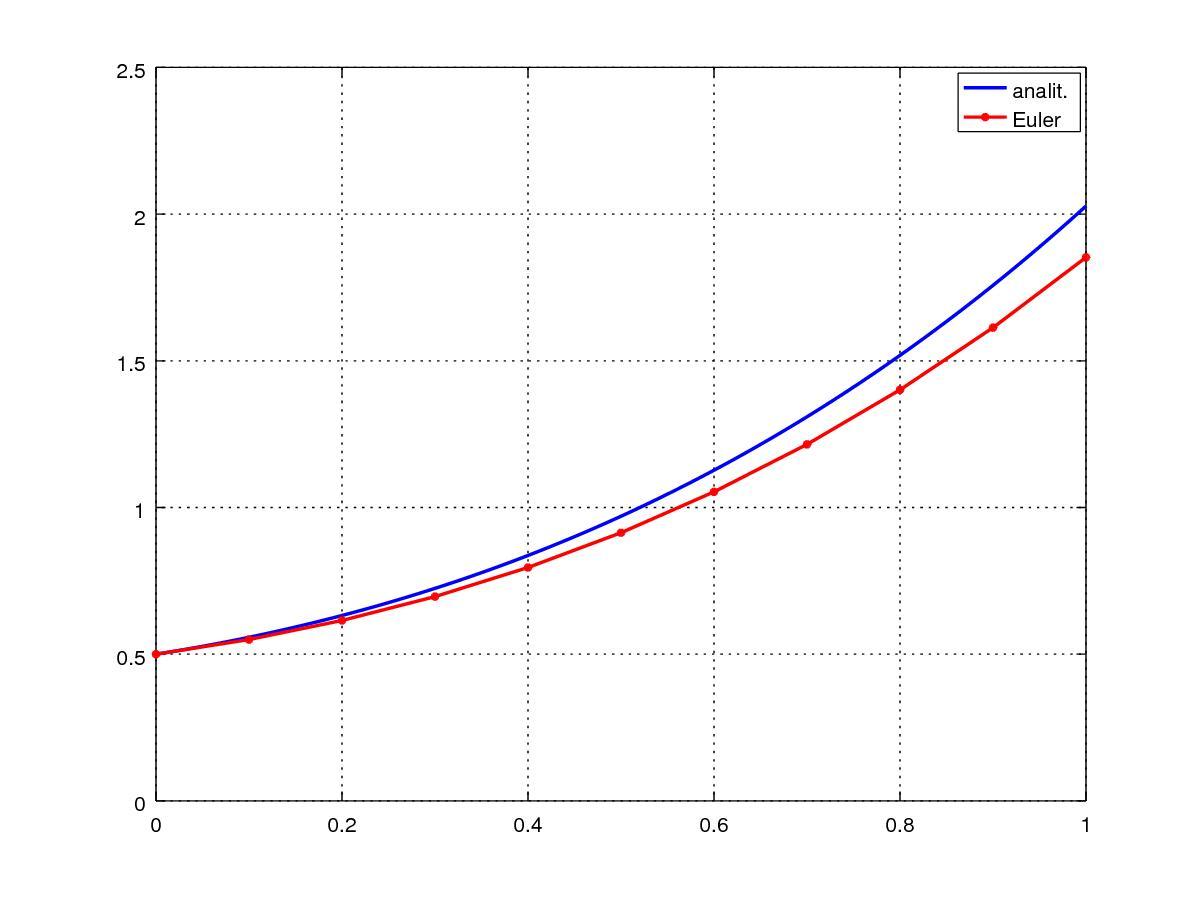
\includegraphics[width=\textwidth]{./cap_pvi/dados/ex_Euler_1/ex_Euler_1}
  \caption{Esboço das soluções referente ao Exemplo~\ref{ex:Euler_1}.}
  \label{fig:ex_Euler_1}
\end{figure}

\ifisoctave
As aproximações obtidas neste exemplo podem ser computadas no \verb+GNU Octave+ com o seguinte código:
\begin{verbatim}
f = @(t,y) y+sin(t);

h=0.1;
n=11;
t=zeros(n,1);
y=zeros(n,1);

t(1)=0;
y(1)=0.5;

for i=1:n-1
  t(i+1) = t(i)+h;
  y(i+1)=y(i)+h*f(t(i),y(i));
endfor

printf("%1.5E %1.5E\n",t(n),y(n))
tt=linspace(0,1);
ya = @(t) exp(t)-sin(t)/2-cos(t)/2;
plot(tt,ya(tt),'b-',...
     t,y,'r.-');grid
legend("analit.","Euler")
\end{verbatim}
\fi
\end{ex}

\subsection{Análise de consistência e convergência}

O método de Euler com passo $h$ aplicado ao problema de valor inicial \eqref{eq:Euler_pvi_1}-\eqref{eq:Euler_pvi_2}, pode ser escrito da seguinte forma
\begin{align}
  \tilde{y}(t^{(1)};h) &= y_0,\label{eq:MPS_1}\\
  \tilde{y}(t^{(i+1)};h) &= \tilde{y}(t^{(i)};h) + h\Phi(t^{(i)},\tilde{y}(t^{(i)});h),\label{eq:MPS_2}
\end{align}
onde $\tilde{y}(t^{(i)})$ representa a aproximação da solução exata $y$ no tempo $t^{(i)}=t_0+(i-1)h$, $i=1, 2, \ldots$. Métodos que podem ser escritos desta forma, são chamados de métodos de passo simples (ou único). No caso específico do método de Euler, temos
\begin{equation}
  \Phi(t,y;h) := f(t,y(t)).
\end{equation}

Agora, considerando a solução exata $y(t)$ de \eqref{eq:Euler_pvi_1}-\eqref{eq:Euler_pvi_2}, introduzimos
\begin{equation}
  \Delta(t,y;h) := \left\{
    \begin{array}{ll}
      \frac{y(t+h)-y(t)}{h} &, h\neq 0,\\
      f(t,y(t)) &, h=0,
    \end{array}\right.
\end{equation}

Com isso, vamos analisar o chamado \emph{erro de discretização local}
\begin{equation}
  \tau(t,y;h) := \Delta(t,y;h) - \Phi(t,y;h),
\end{equation}
a qual estabelece uma medida quantitativa com que a solução exata $y(t)$ no tempo $t+h$ satisfaz a iteração de Euler.

\begin{defn}\normalfont{(Consistência)}\label{defn:pvi_consistencia}
  Um método de passo simples \eqref{eq:MPS_1}-\eqref{eq:MPS_2} é dito consistente quando
  \begin{equation}
    \lim_{h\to 0}\tau(t,y;h) = 0,
  \end{equation}
ou, equivalentemente, quando
\begin{equation}
  \lim_{h\to 0} \Phi(t,y;h) = f(t,y).
\end{equation}
\end{defn}

\begin{obs}
  Da Definição~\ref{defn:pvi_consistencia}, temos que o método de Euler é consistente.
\end{obs}

A \emph{ordem do erro de discretização local} de um método de passo simples \eqref{eq:MPS_1}-\eqref{eq:MPS_2} é dita ser $p$, quando
\begin{equation}
  \tau(t,y;h) = O(h^p).
\end{equation}

Para determinarmos a ordem do método de Euler, tomamos a expansão em série de Taylor da solução exata $y(t)$ em torno de $t$, i.e.
\begin{equation}
  y(t+h) = y(t) + hy'(t) + \frac{h^2}{2}y''(t) + \frac{h^3}{6}y'''(t+\theta h), ~0<\theta<1.
\end{equation}
Como $y(t)=f(t,y(t))$ e assumindo a devida suavidade de $f$, temos
\begin{align}
  y''(t) &= \frac{d}{dt}f(t,y(t)) \\
         &= f_t(t,y) + f_y(t,y)y'\\
         &= f_t(t,y) + f_y(t,y)f(t,y).
\end{align}
Então,
\begin{equation}\label{eq:pvi_delta_aux}
  \Delta(t,y;h) = f(t,y(t)) + \frac{h}{2}[f_t(t,y) + f_y(t,y)f(t,y)] + O(h^2).
\end{equation}
Portanto, para o método de Euler temos
\begin{align}
  \tau(t,y;h) &:= \Delta(t,y;h)-\Phi(t,y;h)\\
              &= \frac{h}{2}[f_t(t,y) + f_y(t,y)f(t,y)] + O(h^2)\\
              &= O(h).
\end{align}
Isto mostra que o método de Euler é um método de ordem $1$.

A análise acima trata apenas da consistência do método de Euler. Para analisarmos a convergência de métodos de passo simples, definimos o \emph{erro de discretização global}
\begin{equation}
  e(t;h_n) := \tilde{y}(t;h_n) - y(t),\quad h_n := \frac{t-t_0}{n}.
\end{equation}
E, com isso, dizemos que o método é \emph{convergente} quando
\begin{equation}
  \lim_{n\to \infty} e(t,h_n) = 0,
\end{equation}
bem como, dizemos que o método tem erro de discretização global de ordem $h^p$ quando $e(t,h_n) = O(h^p)$.

\begin{obs}
  Pode-se mostrar que, assumindo a devida suavidade de $f$, que a ordem do erro de discretização global de um método de passo simples é igual a sua ordem do erro de discretização local (veja, \cite[Cap. 7, Sec. 7.2]{Stoer1993a}). Portanto, o método de Euler é convergente e é de ordem $1$.
\end{obs}

\begin{ex}\label{ex:Euler_1}
  Consideremos o seguinte problema de valor inicial
  \begin{align}
    y' - y &= \sen(t), t>0\label{eq:Euler_aux2}\\
    y(0) &= \frac{1}{2}.
  \end{align}
  Na Tabela~\ref{tab:ex_Euler_2}, temos as aproximações $\tilde{y}(1)$ de $y(1)$ computadas pelo método de Euler com diferentes passos $h$.
 
  \begin{table}[h!]
    \centering
    \begin{tabular}{l|cc}
      $h$ & $\tilde{y}(1)$ & $|\tilde{y}(1)-y(1)|$\\\hline
      $10^{-1}$ & $1,85259$ & $1,7\E-01$ \\
      $10^{-2}$ & $2,00853$ & $1,9\E-02$ \\
      $10^{-3}$ & $2,02549$ & $1,9\E-03$ \\
      $10^{-5}$ & $2,02735$ & $4,8\E-05$ \\
      $10^{-7}$ & $2.02739$ & $1,9\E-07$ \\\hline
    \end{tabular}
    \caption{Resultados referentes ao Exemplo~\ref{ex:Euler_2}}
    \label{tab:ex_Euler_2}
  \end{table}

\ifisoctave
Os resultados mostrados na Tabela~\ref{tab:ex_Euler_2} podem ser computados no \verb+GNU Octave+ com o auxílio do seguinte código:
\begin{verbatim}
f = @(t,y) y+sin(t);

h=1e-2;
n=fix(1/h+1);
t=zeros(n,1);
y=zeros(n,1);

t(1)=0;
y(1)=0.5;

for i=1:n-1
  t(i+1) = t(i)+h;
  y(i+1)=y(i)+h*f(t(i),y(i));
endfor

ya = @(t) exp(t)-sin(t)/2-cos(t)/2;
printf("%1.5E %1.1E\n",y(n),abs(y(n)-ya(1)))
\end{verbatim}
\fi
\end{ex}

\subsection*{Exercícios}

\begin{exer}
  Considere o seguinte problema de valor inicial
  \begin{align}
    y' &+ e^{-y^2+1} = 2,\quad t>1,\\
    y(1) &= -1.
  \end{align}
Use o método de Euler com passo $h=0,1$ para computar o valor aproximado de $y(2)$.
\end{exer}
\begin{resp}
  \ifisoctave 
  \href{https://github.com/phkonzen/notas/blob/master/src/MatematicaNumerica/cap_integr/dados/exer_Euler_pvi1/exer_Euler_pvi1.m}{Código.} 
  \fi
  $-5,87722\E-1$
\end{resp}


\section{Métodos de Runge-Kutta}\label{cap_pvi_sec_RK}

Os métodos de Runge-Kutta de $s$-estágios são métodos de passo simples da seguinte forma
\begin{equation}
  y^{(i+1)} = y^{(i)} + h(c_1k_1 + \cdots + c_sk_s)
\end{equation}
onde
\begin{align}
  k_1 &:= f(t^{(i)},y^{(i)}),\\
  k_2 &:= f(t^{(i)}+\alpha_2h,y^{(i)}+h\beta_{21}k_1),\\
  k_3 &:= f(t^{(i)}+\alpha_3h,y^{(i)}+h(\beta_{31}k_1+\beta_{32}k_2)),\\
      &~~\vdots\\
  k_s &:= f(t^{(i)}+\alpha_sh,y^{(i)}+h(\beta_{s1}k_1+\cdots+\beta_{s,s-1}k_{s-1})),
\end{align}
$t^{(i)}=t_0+(i-1)h$ e $y^{(1)}=y_0$.

Na sequência, discutimos alguns dos métodos de Runge-Kutta usualmente utilizados. Pode-se encontrar uma lista mais completa em~\cite[Cap. 8, Sec. 3.2]{Isaacson1994a}.

\subsection{Métodos de Runge-Kutta de ordem 2}

Precisamos apenas de $2$ estágios para obtermos métodos de Runge-Kutta de ordem 2. Portanto, assumimos
\begin{align}
  y^{(i+1)} = y^{(i)} &+ h\left[c_1f(t^{(i)},y^{(i)}) \right.\nonumber\\
  &\left. + c_2f(t^{(i)}+\alpha_2h,y^{(i)}+h\beta_{21}f(t^{(i)},y^{(i)}))\right].\label{eq:rk_2_aux}
\end{align}
Neste caso, o erro de discretização local é dado por
\begin{equation}
  \tau(t,y;h) = \Delta(t,y;h) - \Phi(t,y;h),
\end{equation}
onde, da equação~\eqref{eq:pvi_delta_aux} temos
\begin{equation}\label{eq:pvi_delta_aux2}
  \Delta(t,y;h) = f(t,y(t)) + \frac{h}{2}[f_t(t,y) + f_y(t,y)f(t,y)] + O(h^2)
\end{equation}
e de~\eqref{eq:rk_2_aux}
\begin{equation}
  \Phi(t,y;h) = c_1f(t,y) + c_2f(t+\alpha_2h,y+h\beta_{21}f(t,y))
\end{equation}
Agora, tomando a expansão de série de Taylor em torno de $t$ de $\Phi(t,y;h)$, temos
\begin{align}\label{eq:pvi_phi_aux2}
  \Phi(t,y;h) = (c_1+c_2)f(t,y) &+ c_2h[\alpha_2f_t(t,y) \nonumber\\
  &+\beta_{21}f_y(t,y)f(t,y)) + O(h^2).
\end{align}
Então, por comparação de \eqref{eq:pvi_delta_aux2} e \eqref{eq:pvi_phi_aux2}, temos
\begin{align}
  c_1&+c_2 = 1\\
  c_2&\alpha_2 = \frac{1}{2}\\
  c_2&\beta_{21} = \frac{1}{2}.
\end{align}
Assim sendo, temos mais de uma solução possível.

\subsubsection{Método do ponto médio}

O método do ponto médio é um método de Runge-Kutta de ordem $2$ proveniente da escolha de coeficientes
\begin{equation}
  c_1 = 0, \quad c_2 = 1, \quad \alpha_2 = \frac{1}{2},\quad \beta_{21}=\frac{1}{2}.
\end{equation}
Logo, a iteração do método do ponto médio é
\begin{align}
  y^{(1)} &= y_0\\
  y^{(i+1)} &= y^{(i)} + hf\left(t^{(i)}+\frac{h}{2},y^{(i)}+\frac{h}{2}f(t^{(i)},y^{(i)}\right).
\end{align}

\begin{ex}\label{ex:ponto_medio_1}
  Consideremos o seguinte problema de valor inicial
  \begin{align}
    y' - y &= \sen(t), t>0\\
    y(0) &= \frac{1}{2}.
  \end{align}
  Na Tabela~\ref{tab:ex_ponto_medio_1}, temos as aproximações $\tilde{y}(1)$ de $y(1)$ computadas pelo método do ponto médio com diferentes passos $h$.
 
  \begin{table}[h!]
    \centering
    \begin{tabular}{l|cc}
      $h$ & $\tilde{y}(1)$ & $|\tilde{y}(1)-y(1)|$\\\hline
      $10^{-1}$ & $2,02175$ & $5,6\E-03$ \\
      $10^{-2}$ & $2,02733$ & $6,0\E-05$ \\
      $10^{-3}$ & $2,02739$ & $6,1\E-07$ \\
      $10^{-4}$ & $2,02740$ & $6,1\E-09$ \\
      $10^{-5}$ & $2,02737$ & $2,9\E-05$ \\\hline
    \end{tabular}
    \caption{Resultados referentes ao Exemplo~\ref{ex:ponto_medio_1}.}
    \label{tab:ex_ponto_medio_1}
  \end{table}

\ifisoctave
Os resultados mostrados na Tabela~\ref{tab:ex_ponto_medio_1} podem ser computados no \verb+GNU Octave+ com o auxílio do seguinte código:
\begin{verbatim}
f = @(t,y) y+sin(t);

h=1e-1;
n=fix(1/h+1);
t=zeros(n,1);
y=zeros(n,1);

t(1)=0;
y(1)=0.5;

for i=1:n-1
  t(i+1) = t(i)+h;
  y(i+1)=y(i)+h*f(t(i)+h/2,y(i)+h/2*f(t(i),y(i)));
endfor

ya = @(t) exp(t)-sin(t)/2-cos(t)/2;
printf("%1.5E %1.1E\n",y(n),abs(y(n)-ya(1)))
\end{verbatim}
\fi
\end{ex}

\subsubsection{Método de Euler modificado}

O método de Euler modificado é um método de Runge-Kutta de ordem $2$ proveniente da escolha de coeficientes
\begin{equation}
  c_1 = \frac{1}{2}, \quad c_2 = \frac{1}{2}, \quad \alpha_2 = 1,\quad \beta_{21}=1.
\end{equation}
Logo, a iteração do método de Euler modificado é
\begin{align}
  y^{(1)} &= y_0\\
  y^{(i+1)} &= y^{(i)} + \frac{h}{2}\left[f(t^{(i)},y^{(i)}) + f(t^{(i)}+h,y^{(i)}+hf(t^{(i)},y^{(i)})\right].
\end{align}

\begin{ex}\label{ex:Euler_modificado_1}
  Consideremos o seguinte problema de valor inicial
  \begin{align}
    y' - y &= \sen(t), t>0\\
    y(0) &= \frac{1}{2}.
  \end{align}
  Na Tabela~\ref{tab:ex_Euler_modificado_1}, temos as aproximações $\tilde{y}(1)$ de $y(1)$ computadas pelo método de Euler modificado com diferentes passos $h$.
 
  \begin{table}[h!]
    \centering
    \begin{tabular}{l|cc}
      $h$ & $\tilde{y}(1)$ & $|\tilde{y}(1)-y(1)|$\\\hline
      $10^{-1}$ & $2,02096$ & $6,4\E-03$ \\
      $10^{-2}$ & $2,02733$ & $6,9\E-05$ \\
      $10^{-3}$ & $2,02739$ & $6,9\E-07$ \\
      $10^{-4}$ & $2,02740$ & $6,9\E-09$ \\
      $10^{-5}$ & $2.02737$ & $2,9\E-05$ \\\hline
    \end{tabular}
    \caption{Resultados referentes ao Exemplo~\ref{ex:Euler_modificado_1}}
    \label{tab:ex_Euler_modificado_1}
  \end{table}

\ifisoctave
Os resultados mostrados na Tabela~\ref{tab:ex_Euler_modificado_1} podem ser computados no \verb+GNU Octave+ com o auxílio do seguinte código:
\begin{verbatim}
f = @(t,y) y+sin(t);

h=1e-1;
n=fix(1/h+1);
t=zeros(n,1);
y=zeros(n,1);

t(1)=0;
y(1)=0.5;

for i=1:n-1
  t(i+1) = t(i)+h;
  y(i+1)=y(i)+h*f(t(i),y(i));
  y(i+1)=y(i)+h/2*(f(t(i),y(i))+f(t(i+1),y(i+1)));
endfor

ya = @(t) exp(t)-sin(t)/2-cos(t)/2;
printf("%1.5E %1.1E\n",y(n),abs(y(n)-ya(1)))
\end{verbatim}
\fi
\end{ex}

\subsection{Método de Runge-Kutta de ordem $4$}

Um dos métodos de Runge-Kutta mais empregados é o seguinte método de ordem $4$:
\begin{equation}
  y^{(i+1)} = y^{(i)} + \frac{h}{6}(k_1 + 2k_2 + 2k_3 + k_4),
\end{equation}
onde
\begin{align}
  k_1 &:= f(t^{(i)},y^{(i)}),\\
  k_2 &:= f(t^{(i)}+h/2,y^{(i)}+hk_1/2),\\
  k_3 &:= f(t^{(i)}+h/2,y^{(i)}+hk_2/2),\\
  k_4 &:= f(t^{(i)}+h,y^{(i)}+hk_3),
\end{align}
$t^{(i)}=t_0+(i-1)h$ e $y^{(1)}=y_0$.

\begin{ex}\label{ex:RK4_1}
  Consideremos o seguinte problema de valor inicial
  \begin{align}
    y' - y &= \sen(t), t>0\\
    y(0) &= \frac{1}{2}.
  \end{align}
  Na Tabela~\ref{tab:ex_RK4_1}, temos as aproximações $\tilde{y}(1)$ de $y(1)$ computadas pelo método de Runge-Kutta de quarta ordem com diferentes passos $h$.
 
  \begin{table}[h!]
    \centering
    \begin{tabular}{l|cc}
      $h$ & $\tilde{y}(1)$ & $|\tilde{y}(1)-y(1)|$\\\hline
      $10^{-1}$ & $2,02739$ & $2,8\E-06$ \\
      $10^{-2}$ & $2,02740$ & $3,1\E-10$ \\
      $10^{-3}$ & $2,02740$ & $3,0\E-14$ \\
      $10^{-4}$ & $2,02740$ & $4,4\E-14$ \\\hline
    \end{tabular}
    \caption{Resultados referentes ao Exemplo~\ref{ex:RK4_1}}
    \label{tab:ex_RK4_1}
  \end{table}

\ifisoctave
Os resultados mostrados na Tabela~\ref{tab:ex_RK4_1} podem ser computados no \verb+GNU Octave+ com o auxílio do seguinte código:
\begin{verbatim}
f = @(t,y) y+sin(t);

h=1e-4;
n=fix(1/h+1);
t=zeros(n,1);
y=zeros(n,1);

t(1)=0;
y(1)=0.5;

for i=1:n-1
  t(i+1) = t(i)+h;
  k1 = h*f(t(i),y(i));
  k2 = h*f(t(i)+h/2,y(i)+k1/2);
  k3 = h*f(t(i)+h/2,y(i)+k2/2);
  k4 = h*f(t(i)+h,y(i)+k3);
  y(i+1)=y(i)+(k1+2*k2+2*k3+k4)/6;
endfor

ya = @(t) exp(t)-sin(t)/2-cos(t)/2;
printf("%1.5E %1.1E\n",y(n),abs(y(n)-ya(1)))
\end{verbatim}
\fi
\end{ex}

\subsection{Exercícios}

\begin{exer}
  Considere o seguinte problema de valor inicial
  \begin{align}
    y' &+ e^{-y^2+1} = 2,\quad t>1,\\
    y(1) &= -1.
  \end{align}
Use os seguintes métodos de Runge-Kutta com passo $h=0,1$ para computar o valor aproximado de $y(2)$:
\begin{enumerate}[a)]
\item método do ponto médio.
\item método de Euler modificado.
\item método de Runge-Kutta de ordem $4$.
\end{enumerate}
\end{exer}
\begin{resp}
  \ifisoctave 
  \href{https://github.com/phkonzen/notas/blob/master/src/MatematicaNumerica/cap_integr/dados/exer_RK_pvi1/exer_RK_pvi1.m}{Código.} 
  \fi
  a)~$-6,00654\E-1$; b)~$-6,00703\E-1$; c)~$-5,99608\E-1$
\end{resp}

%Este trabalho está licenciado sob a Licença Atribuição-CompartilhaIgual 4.0 Internacional Creative Commons. Para visualizar uma cópia desta licença, visite http://creativecommons.org/licenses/by-sa/4.0/deed.pt_BR ou mande uma carta para Creative Commons, PO Box 1866, Mountain View, CA 94042, USA.

\chapter{Problema de valor de contorno}\label{cap_pvc}
\thispagestyle{fancy}

Neste capítulo, discutimos sobre a aplicação do método de diferenças finitas para aproximar a solução de problemas de valores de contorno da forma
\begin{align}
  \alpha(x) u'' &+ \beta(x) u' + \gamma(x) u = f(x),\quad c_1 < x < c_2,\\
  \eta_1 u'(c_1) &+ \theta_1 u(c_1) = g_1\\
  \eta_2 u'(c_2) &+ \theta_2 u(c_2) = g_2
\end{align}
onde a incógnita $u = u(x)$ e os são dados os coeficientes $\alpha(x)\neq 0$, $\beta(x)$, $\gamma(x)$ e a função $f(x)$. Nas condições de contorno, são dados os coeficientes $\eta_1$ e $\theta_1$ não simultaneamente nulos, bem como, os coeficientes $\eta_2$ e $\theta_2$, também, não simultaneamente nulos.

\section{Método de diferenças finitas}\label{cap_pvc_sec_mdf}

Consideramos o seguinte problema linear de valor de contorno
\begin{align}
  \alpha(x) u'' &+ \beta(x) u' + \gamma(x) u = f(x),\quad c_1 < x < c_2, \label{eq:pvc_eq}\\
  \eta_1 u'(c_1) &+ \theta_1 u(c_1) = g_1 \label{eq:pvc_bc1}\\
  \eta_2 u'(c_2) &+ \theta_2 u(c_2) = g_2 \label{eq:pvc_bc2}
\end{align}
onde a incógnita $u = u(x)$ e os são dados os coeficientes $\alpha(x)\neq 0$, $\beta(x)$, $\gamma(x)$ e a função $f(x)$. Nas condições de contorno, são dados os coeficientes $\eta_1$ e $\theta_1$ não simultaneamente nulos, bem como, os coeficientes $\eta_2$ e $\theta_2$, também, não simultaneamente nulos.

A aproximação pelo método de diferenças finitas de \eqref{eq:pvc_eq}-\eqref{eq:pvc_bc2} surge da substituição das derivadas por fórmulas de diferenças finitas. Isto requer a a prévia discretização do domínio do problema. Mais precisamente, a aplicação do método de diferenças finitas envolve três procedimentos básicos: 1. discretização do domínio, 2. discretização das equações, 3. resolução do problema discreto.

\begin{flushleft}
  {\bf 1. Discretização do domínio}
\end{flushleft}

A discretização do domínio refere-se ao particionamento do mesmo em pontos espaçados uniformemente ou não. Aqui, para mantermos a simplicidade, vamos considerar apenas o caso de um particionamento uniforme. Desta forma, escolhemos o número $n$ de pontos da partição e, então, o passo é dado por
\begin{equation}
  h = \frac{c_2-c_1}{n-1},
\end{equation}
e os pontos da partição podem ser indexados da seguinte forma
\begin{equation}
  x_i = c_1 + (i-1)h.
\end{equation}

\begin{flushleft}
  {\bf 2. Discretização das equações}
\end{flushleft}

Começando pela equação \eqref{eq:pvc_eq}, no ponto $x=x_i$ temos
\begin{equation}
  \alpha(x_i) u''(x_i) + \beta(x_i) u'(x_i) + \gamma(x_i) u(x_i) = f(x_i) \label{eq:pvc_eq_no_ponto}
\end{equation}
para $i=2, 3, \dotsc, n-1$. Podemos substituir a segunda derivada de $u$ pela fórmula de diferenças finitas central de ordem $h^2$, i.e.
\begin{equation}
  u''(x_i) = \underbrace{\frac{u(x_i-h) - 2u(x_i) + u(x_i+h)}{h^2}}_{D_{0,h^2}^2u(x_i)} + O(h^2).
\end{equation}
A primeira derivada de $u$ também pode ser substituída pela fórmula de diferenças finitas central de ordem $h^2$, i.e.
\begin{equation}
  u'(x_i) = \underbrace{\frac{u(x_i+h)-u(x_i-h)}{2h}}_{D_{0,h^2}u(x_i)} + O(h^2).
\end{equation}

Agora, denotando $u_i \approx u(x_i)$, temos $u_{i-1}\approx u(x_i-h)$ e $u_{i+1}\approx u(x_i+h)$. Então, substituindo as derivadas pelas fórmulas de diferenças finitas acima na equação \eqref{eq:pvc_eq_no_ponto}, obtemos
\begin{align}
  \alpha(x_i)\left(\frac{u_{i-1}-2u_i+u_{i+1}}{h^2}\right) &+ \beta(x_i)\left(\frac{u_{i+1}-u_{i-1}}{2h}\right) \nonumber \\
  &+ \gamma(x_i)u_i + O(h^2) = f(x_i),
\end{align}
para $i=2, 3, \dotsc, n-1$. Rearranjando os termos e desconsiderando o termo do erro de truncamento, obtemos o seguinte sistema discreto de equações lineares
\begin{align}
  \left(\frac{\alpha(x_i)}{h^2}-\frac{\beta(x_i)}{2h}\right)u_{i-1} &+ \left(\gamma(x_i) - \frac{2\alpha(x_i)}{h^2}\right)u_i \nonumber \\
  &+ \left(\frac{\alpha(x_i)}{h^2}+\frac{\beta(x_i)}{2h}\right)u_{i+1} = f(x_i), \label{eq:pvc_mdf_sis1}
\end{align}
para $i=2, 3, \dotsc, n-1$. Observe que este sistema consiste em $n-2$ equações envolvendo as $n$ incógnitas $u_i$, $i=1, 2, \dotsc, n$. Para fechá-lo, usamos as condições de contorno.

Usando a fórmula de diferenças finitas progressiva de ordem $h^2$ para a derivada $u'(c_1)$ temos
\begin{equation}
  u'(c_1) = \frac{-3u(c_1) + 4u(c_1+h) - u(c_1+2h}{2h} + O(h^2).
\end{equation}
Então, observando que $c_1$ corresponde ao ponto $x_1$ na partição do domínio, temos $u_1 \approx u(c_1)$, $u_2 = u(c_1+h)$ e $u_3 = u(c_1+2h)$ e, portanto de \eqref{eq:pvc_bc1} temos
\begin{equation}
  \eta_1\left(\frac{-3u_1 + 4u_2 - u_3}{2h}\right) + \theta_1u_1 + O(h^2) = g_1.
\end{equation}
Então, desconsiderando o termo do erro de truncamento, obtemos a seguinte equação discreta
\begin{equation}
  \left(\theta_1 - \frac{3\eta_1}{2h}\right)u_1 + \frac{2\eta_1}{h}u_2 - \frac{\eta_1}{2h}u_3 = g_1.\label{eq:pvc_mdf_sis0}
\end{equation}

Procedendo de forma análoga para a condição de contorno \eqref{eq:pvc_bc2}, usamos a fórmula de diferenças finitas regressiva de ordem $h^2$ para a derivada $u'(c_2)$, i.e.
\begin{equation}
  u'(c_2) = \frac{3u(c_2) - 4u(c_2-h)+u(c_2-2h)}{2h} + O(h^2).
\end{equation}
Aqui, temos $u_{n}\approx u(c_2)$, $u_{n-1}\approx u(c_2-h)$ e $u_{n-2}\approx u(c_2-2h)$, e de \eqref{eq:pvc_bc2} obtemos
\begin{equation}
  \eta_2\left(\frac{3u_n - 4u_{n-1} + u_{n-2}}{2h}\right) + \theta_2u_n + O(h^2) = g_2.
\end{equation}
Então, desconsiderando o termo do erro de truncamento, obtemos
\begin{equation}
  \frac{\eta_2}{2h}u_{n-2} - \frac{2\eta_2}{h}u_{n-1} + \left(\theta_2 + \frac{3\eta_2}{2h}\right)u_n = g_2.\label{eq:pvc_mdf_sis2}
\end{equation}

Por fim, as equações \eqref{eq:pvc_mdf_sis0}-\eqref{eq:pvc_mdf_sis2} formam o seguinte problema discretizado pelo método de diferenças finitas
\begin{align}
  &\left(\theta_1 - \frac{3\eta_1}{2h}\right)u_1 + \frac{2\eta_1}{h}u_2 - \frac{\eta_1}{2h}u_3 = g_1.\label{eq:pvc_mdf_bc1}\\
  &~\nonumber\\
  &\left(\frac{\alpha(x_i)}{h^2}-\frac{\beta(x_i)}{2h}\right)u_{i-1} + \left(\gamma(x_i) - \frac{2\alpha(x_i)}{h^2}\right)u_i \nonumber \\
  &+ \left(\frac{\alpha(x_i)}{h^2}+\frac{\beta(x_i)}{2h}\right)u_{i+1} = f(x_i),~i=2, \dotsc, n-1, \label{eq:pvc_mdf_eq}\\
  &~\nonumber\\
  &\frac{\eta_2}{2h}u_{n-2} - \frac{2\eta_2}{h}u_{n-1} + \left(\theta_2 + \frac{3\eta_2}{2h}\right)u_n = g_2.\label{eq:pvc_mdf_bc2}
\end{align}

\begin{flushleft}
  {\bf 3. Resolução do problema discreto}
\end{flushleft}

O problema discreto \eqref{eq:pvc_mdf_bc1}-\eqref{eq:pvc_mdf_bc2} consiste em um sistema linear de $n$ equações com $n$ incógnitas. Na forma matricial temos
\begin{equation}
  A\tilde{u} = b
\end{equation}
onde $\tilde{u} = (u_1, u_2, \dotsc, u_n)$ é o vetor das incógnitas, $b$ é o vetor dos termos contantes $b = (g_1, f(x_2), f(x_3), \dotsc, f(x_{n-1}), g_2)$ e $A$ é a matriz dos coeficientes. Observamos que os coeficientes não nulos da matriz $A$ são:
\begin{align}
  a_{11} &= \left(\theta_1 - \frac{3\eta_1}{2h}\right),\\
  a_{12} &= \frac{2\eta_1}{h},\\
  a_{13} &= - \frac{\eta_1}{2h},\\
  & ~ \nonumber \\
  a_{i,i-1} &= \left(\frac{\alpha(x_i)}{h^2}-\frac{\beta(x_i)}{2h}\right), ~i=2, \dotsc, n-1,\\
  a_{i,i} &= \left(\gamma(x_i) - \frac{2\alpha(x_i)}{h^2}\right), ~i=2, \dotsc, n-1, \\
  a_{i,i+1} &= \left(\frac{\alpha(x_i)}{h^2}+\frac{\beta(x_i)}{2h}\right), ~i=2, \dotsc, n-1,\\
  & ~ \nonumber \\
  a_{n,n-2} &= \frac{\eta_2}{2h},\\
  a_{n,n-1} &= - \frac{2\eta_2}{h},\\
  a_{n,n} &= \left(\theta_2 + \frac{3\eta_2}{2h}\right).
\end{align}
Com isso em mente, a matriz $A$ tem a seguinte estrutura
\begin{equation}
  A = \begin{bmatrix}
    a_{11} & a_{12} & a_{13} \\
    a_{21} & a_{22} & a_{23} \\
      & \ddots  & \ddots & \ddots \\
      & & a_{i,i-1} & a_{i,i} & a_{i,i+1} \\
      & & \ddots  & \ddots & \ddots \\
      & & & a_{n-1,n-2} & a_{n-1,n-1} & a_{n-1,n} \\
      & & & a_{n,n-2} & a_{n,n-1} & a_{n,n}
  \end{bmatrix}.
\end{equation}

A resolução do sistema discreto se resume, então, a resolver o sistema $A\tilde{u} = b$, o que pode ser feito por qualquer método numérica apropriada.


\begin{ex}\label{ex:pvc_mdf_1}
  Consideremos o seguinte problema de valor de contorno
  \begin{align}
    -u'' &= \sen(x),\quad 0\leq x \leq 2,\\
    u(0) &= 0,\\
    u(1) &= \sen(2).
  \end{align}

\begin{figure}[h!]
  \centering
  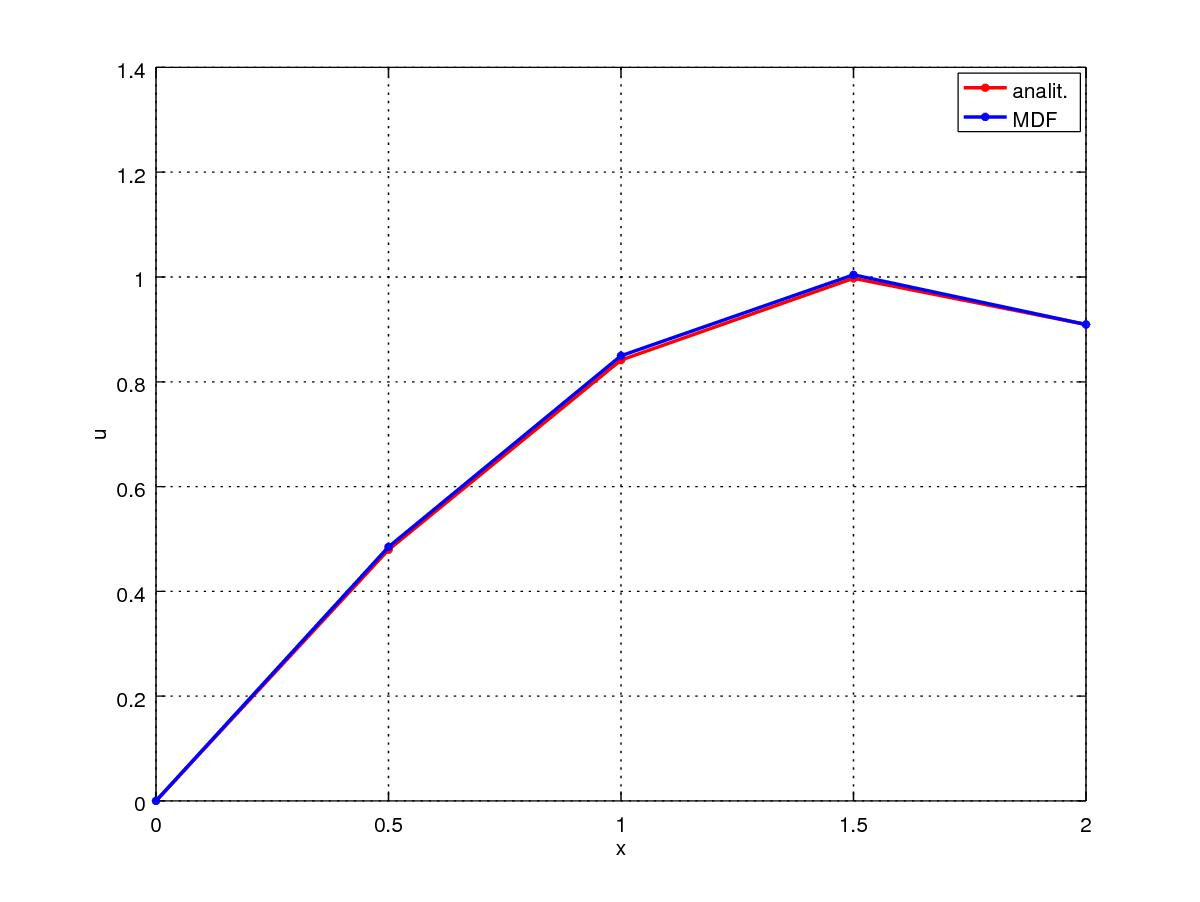
\includegraphics[width=0.8\textwidth]{./cap_pvc/dados/ex_pvc_mdf_1/ex_pvc_mdf_1}
  \caption{Resultado referente ao Exemplo~\ref{ex:pvc_mdf_1}.}
  \label{fig:ex_pvc_mdf_1}
\end{figure}

A solução analítica deste problema é $u(x) = \sen(x)$. Agora, usando a abordagem pelo método de diferenças finitas abordado nesta seção, obtemos o seguinte problema discreto
\begin{align}
  u_1 &= 0,\\
  -\frac{1}{h^2}u_{i-1} + \frac{2}{h^2}u_i - \frac{1}{h^2}u_{i+1} &= \sen(x_i),~i=2, \dotsc, n-1,\\
  u_n = \sen(2),
\end{align}
onde $h=\pi/(n-1)$ e $x_i = (i-1)h$.

\begin{table}[h!]
  \centering
  \begin{tabular}{ll|c}
    $h$ & $n$ & $\|\tilde{u} - u\|_{L^2}$ \\\hline
    $10^{-1}$ & $21$ & $1,0\E-03$ \\
    $10^{-2}$ & $201$ & $3,3\E-05$ \\
    $10^{-3}$ & $2001$ & $1,0\E-06$ \\\hline
  \end{tabular}
  \caption{Resultados referentes ao Exemplo~\ref{ex:pvc_mdf_1}.}
  \label{tab:ex_pvc_mdf_1}
\end{table}

Resolvendo este sistema com $h=0,5$ obtemos a solução numérica apresentada na Figura~\ref{fig:ex_pvc_mdf_1}. Ainda, na Tabela~\ref{tab:ex_pvc_mdf_1} temos a comparação na norma $L^2$ da solução numérica $\tilde{u} = (u_1, u_2, \dotsc, u_n)$ com a solução analítica $u(x)=\sen(x)$ para diferentes escolhas de $h$.

\ifisoctave
No \verb+GNU Octave+, podemos computar os resultados discutidos neste exemplo com o seguinte código:
\begin{verbatim}
#param
n = 5;
h = 2/(n-1);

#fonte
f = @(x) sin(x);

#nodos
x = linspace(0,2,n)';

#sist. MDF
A = zeros(n,n);
b = zeros(n,1);

A(1,1) = 1;
b(1)=0;
for i=2:n-1
  A(i,i-1)=-1/h^2;
  A(i,i)=2/h^2;
  A(i,i+1)=-1/h^2;
  b(i)=sin(x(i));
endfor
A(n,n)=1;
b(n)=sin(2);

#sol MDF
u = A\b;

#sol. analic.
ua = @(x) sin(x);

#grafico comparativo
plot(x,ua(x),'r.-',...
     x,u,'b.-');grid
legend("analit.","MDF")
xlabel("x")
ylabel("u")

#erro na norma L2
printf("%1.1E %1.1E\n", h,norm(u-ua(x)))
\end{verbatim}
\fi
\end{ex}

\subsection*{Exercícios}

\begin{exer}
Considere o seguinte problema de valor inicial
  \begin{align}
    -u'' &+ u' = f(x),~-1<x<1,\\
    u(-1)&=0,\\
    u'(1)&=0,
  \end{align}
  onde
  \begin{equation}
    f(x) = \left\{
      \begin{array}{ll}
        1 &, x\leq 0\\
        0 &, x>0
      \end{array}
    \right.
  \end{equation}
\end{exer}
Use uma aproximação adequada pelo método de diferenças finitas para obter o valor aproximado de $u(0)$ com precisão de $2$ dígitos significativos.
\begin{resp}
  \ifisoctave 
  \href{https://github.com/phkonzen/notas/blob/master/src/MatematicaNumerica/cap_pvc/dados/exer_pvc_mdf_1/exer_pvc_mdf_1.m}{Código.} 
  \fi
  $7,2\E-1$
\end{resp}


%resposta dos exercícios
\ifisbook
%Este trabalho está licenciado sob a Licença Atribuição-CompartilhaIgual 4.0 Internacional Creative Commons. Para visualizar uma cópia desta licença, visite http://creativecommons.org/licenses/by-sa/4.0/ ou mande uma carta para Creative Commons, PO Box 1866, Mountain View, CA 94042, USA.

\chapter*{Resposta dos Exercícios}\label{c_respostas}
\addcontentsline{toc}{chapter}{Respostas dos Exercícios}

\shipoutAnswer
\fi

%references
\nocite{*}
\bibliographystyle{plain}
\bibliography{main}
\addcontentsline{toc}{chapter}{Referências Bibliográficas}

\ifisbook
\clearpage
\addcontentsline{toc}{chapter}{Índice Remissivo}
\printindex
\fi

\end{document}
